\documentclass[a4paper,12pt]{article}

% -------------------------------------------------
% CODIFICA E LINGUA
% -------------------------------------------------

\usepackage[utf8]{inputenc}   % Codifica UTF-8
\usepackage[T1]{fontenc}      % Font encoding
\usepackage[italian]{babel}   % Lingua italiana

% -------------------------------------------------
% MATEMATICA
% -------------------------------------------------

\usepackage{amsmath}
\usepackage{amssymb}
\usepackage{hyperref}
\usepackage{amsthm}
\usepackage{mathtools}
\usepackage{bm}               % Bold math symbols
\usepackage{physics}          % Derivate, norme, bra-ket, ecc.
\usepackage{mathrsfs}         % Font calligrafico
\usepackage{esint}            % Integrali particolari

% -------------------------------------------------
% TEOREMI, DEFINIZIONI, ECC.
% -------------------------------------------------

\newtheorem{theorem}{Teorema}[section]
\newtheorem{lemma}[theorem]{Lemma}
\newtheorem{proposition}[theorem]{Proposizione}
\newtheorem{corollary}[theorem]{Corollario}

\theoremstyle{definition}
\newtheorem{definition}[theorem]{Definizione}
\newtheorem{example}[theorem]{Esempio}
\newtheorem{remark}[theorem]{Osservazione}

% -------------------------------------------------
% GRAFICA E IMMAGINI
% -------------------------------------------------

\usepackage{graphicx}
\usepackage{float}
\usepackage{subcaption}
\usepackage{caption}

% Percorso immagini (opzionale)
% \graphicspath{{images/}}

% -------------------------------------------------
% TABELLE
% -------------------------------------------------

\usepackage{booktabs}
\usepackage{array}
\usepackage{multirow}
\usepackage{csvsimple}

% -------------------------------------------------
% COLORI E LINK
% -------------------------------------------------

\usepackage{xcolor}

\usepackage[nameinlink]{cleveref}

% -------------------------------------------------
% GEOMETRIA PAGINA
% -------------------------------------------------

\usepackage[a4paper,margin=2.7cm]{geometry}

% -------------------------------------------------
% BIBLIOGRAFIA
% -------------------------------------------------

\usepackage[backend=bibtex, style=numeric]{biblatex}
\addbibresource{bibliografia.bib} 

% -------------------------------------------------
% LISTE
% -------------------------------------------------

\usepackage{enumitem}

% -------------------------------------------------
% CODICE
% -------------------------------------------------

\usepackage{listings}
\usepackage{minted}
\usepackage[linesnumbered,ruled,vlined]{algorithm2e}

\lstset{
    basicstyle=\ttfamily\small,
    breaklines=true,
    frame=single,
    numbers=left,
    numberstyle=\tiny,
    showstringspaces=false
}

% -------------------------------------------------
% TIKZ (diagrammi e grafici)
% -------------------------------------------------

\usepackage{tikz}
\usetikzlibrary{
    arrows.meta,
    positioning,
    calc,
    decorations.pathreplacing
}

% -------------------------------------------------
% HEADER E FOOTER
% -------------------------------------------------

\usepackage{fancyhdr}

\pagestyle{fancy}
\fancyhf{}
\rhead{\thepage}
\lhead{Progetto MNAPDE}

% -------------------------------------------------
% COMANDI PERSONALIZZATI
% -------------------------------------------------

\newcommand{\R}{\mathbb{R}}
\newcommand{\N}{\mathbb{N}}
\newcommand{\Z}{\mathbb{Z}}
\newcommand{\Q}{\mathbb{Q}}
\newcommand{\C}{\mathbb{C}}

% -------------------------------------------------
% TITOLO
% -------------------------------------------------

\title{
    \textbf{Progetto MNAPDE}
}

\author{
    Andrea Cima
}

\date{\today}

% -------------------------------------------------
% DOCUMENTO
% -------------------------------------------------

\begin{document}

\maketitle

\tableofcontents

\newpage

\section{Metodo BEM}
\label{sec:BEM_base}
Studiamo il problema di diffusione di un'onda incidente da parte di un ostacolo poligonale $\Gamma$ nel piano mediante il \textit{Boundary Element Method} (BEM). In particolare, il problema che vogliamo risolvere è il seguente:\\
\vspace{0.7cm}
\begin{minipage}{0.3\textwidth}
\centering
\begin{tikzpicture}

\fill[gray!30] (0,0) -- (2,0.5) -- (1.5,2) -- (0.5,1.8) -- cycle;
\draw[thick] (0,0) -- (2,0.5) -- (1.5,2) -- (0.5,1.8) -- cycle;

\node at (2,2) {$\Omega_+$};
\node at (1.8,1) {$\Gamma$};
\node at (1,1) {$\Omega_-$};

\end{tikzpicture}
\end{minipage}
\hfill
\begin{minipage}{0.55\textwidth}
\begin{equation}
\label{eq:edp}
\begin{cases}
\Delta u^{scat} + k^2u^{scat} = 0 & \text{su } \Omega_+\\
\gamma^+u^{scat} = -\gamma^+ u^{inc} =: g_D & \text{su } \Gamma\\
\text{SRC}
\end{cases}
\end{equation}
\end{minipage}

L'obiettivo è implementare numericamente la formulazione integrale del problema e analizzare il comportamento della soluzione ottenuta al variare della discretizzazione del problema. \\
Calcoliamo il campo scatterato attraverso una formula di rappresentazione tramite il \textit{single layer potential} $\mathcal{S}$, ovvero:
\begin{equation}
    \label{eq:single_layer}
    u^{scat}(x) = \mathcal{S}\psi(x):=\int_\Gamma \Phi_k(x, y)\,\psi(y) \, ds(y) \quad x \in \Omega_+, \psi \in H^{-\frac{1}{2}}(\Gamma).
\end{equation}
Imponendo che $u^{scat}$ soddisfi il problema \ref{eq:edp}, si trova che $\psi$ deve soddisfare:
\begin{equation}
    \label{eq:bie}
    S\psi=g_D,
\end{equation}
in cui $S$ è il \textit{single layer operator} definito come 
\begin{equation}
    \label{eq:slo}
    S\psi(x):=\int_\Gamma \Phi_k(x, y)\,\psi(y) \, ds(y) \quad x \in \Gamma, \psi \in H^{-\frac{1}{2}}(\Gamma),
\end{equation}
dove $g_D$ è il dato del problema \ref{eq:edp}.\\
Per approssimare la soluzione dell'equazione \ref{eq:bie} e trovare la densità $\psi$ viene usato il metodo di collocazione ed una formula di quadratura per il calcolo degli integrali.\\
In particolare vengono fissati:
\begin{align*}
    &V_N \subset H^{-\frac{1}{2}}(\Gamma); \quad \dim V_N = N < + \infty; \quad V_N = \text{span} \{\varphi_1, \dots, \varphi_N\}\\\\
    &\{K_1, \dots, K_N\}: \text{ elementi che partizionano il bordo } \Gamma\\\\
    & \{p_0, \dots, p_N\} \subset \Gamma : \text{estremi degli elementi } \{K_i\} \text{ tali che } p_0=p_N\\\\
    &\{x_1, \dots, x_N\} \subset \Gamma \text{ nodi di collocazione (considero i punti medi di } \{K_1, \dots, K_N\}) \\\\
    & \varphi_j = 
    \begin{cases}
        1 & \text{su } K_j\\
        0 & \text{su } \Gamma \setminus K_j
    \end{cases}
    \qquad \forall j=1, \dots, N.
\end{align*}
I passaggi principali del metodo di collocazione BEM sono:
\begin{enumerate}
    \item costruire la struttura geometrica del problema; ad esempio fissare i nodi di collocazione in modo che siano equi-distribuiti su tutto $\Gamma$;
    \item assemblare la matrice del sistema lineare e il termine noto;
    \item risolvere il sistema lineare per trovare la densità $\psi$;
    \item usare la formula di rappresentazione dell'equazione \ref{eq:single_layer} per trovare l'espressione di $u^{scat}$.
\end{enumerate}

\begin{algorithm}[H]
\caption{Costruzione della Geometria}
\label{alg:1}
\KwIn{Vertici $v$, numero d'onda $k$, numero gradi di libertà $N$, angolo $\theta$ onda piana incidente}
Definisci $\Gamma$ tramite i vertici: $v \leftarrow [v, v_1]$\;
Calcola $side\_length_i = |v_{i+1} - v_i|$ e $perimeter = \sum side\_length_i$\;
$N\_side \leftarrow \lceil N \cdot (side\_length / perimeter) \rceil$\;
\ForEach{lato $i$}{
    Genera punti $p_k^i$ equispaziati su $[v_i, v_{i+1}]$\;
    $x_k^i \leftarrow$ punti medi di di ogni elemento $K_k^i$ \;
    $\tau_k^i \leftarrow$ versore tangente del lato $i$\;
    $h_k^i \leftarrow$ lunghezza del singolo elemento\;
}
Concatena $x_k, p_k, h_k, \tau_k$ eliminando le sovrapposizioni agli angoli\;
\end{algorithm}
Osserviamo che con questa struttura riusciamo a scegliere il numero di nodi di collocazione su ciascun lato in funzione della lunghezza del lato stesso. Inoltre osserviamo che il numero complessivo di nodi di collocazione può essere (leggermente) superiore al numero di gradi di libertà $N$ che abbiamo in input. Nel caso in cui volessimo effettuare dei test con un numero fissato di gradi di libertà, dobbiamo assicurarci che tale numero non venga aumentato dall'algoritmo \ref{alg:1}. 
\vspace{0.5cm}

\begin{algorithm}[H]
\caption{Assemblaggio e Risoluzione}
\label{alg:2}
\KwIn{Punti medi $x_k$, mesh $h_k$, tangenti $\tau_k$}
Calcola $F = - \exp(i k \cdot \mathcal{R}(x_k \cdot e^{-i \theta}))$ e inizializza matrice $A \in \mathbb{C}^{N \times N}$\;
Calcola nodi e pesi di quadratura $(x_q, w_q)$ su $[0, 1]$\;
Scala i nodi su ogni elemento $K_i$\;
\ForEach{$j \in \{1, \dots, N\}$}{
    $y_q \leftarrow p_k + h_k \cdot x_q \cdot \tau_k$\;
    $A_{j,:} \leftarrow \sum \frac{i}{4} H_0^{(1)}(k|x_k(j) - y_q|) \cdot h_k \cdot w_q$\;
}
\tcc{Correzione termini diagonali}
Calcola nuovi nodi e pesi di quadratura $(x_q, w_q)$ su $[0, 1]$\;

\ForEach{$j \in \{1, \dots, N\}$}{
    $y_q \leftarrow \frac{h_k}{2} \cdot x_q$\;
    $A_{j, j} \leftarrow \frac{i}{2}\cdot \frac{h_k(j)}{2} \cdot w_q\cdot H_0^{(1)}(k|y_q|)$
}
$\psi \leftarrow A \setminus F$ \tcp*{Risoluzione sistema lineare}
\end{algorithm}
\vspace{0.5cm}

\begin{algorithm}[H]
\caption{Formula di rappresentazione}
\label{alg:3}
\KwIn{Vettore $\psi$, mesh $p_k, h_k, \tau_k$}
Crea griglia $Z = X + iY$ ed escludi i punti in $\Omega_-$\;
Inizializza $u_{scat}$ ad una matrice di zeri\;
Calcola nuovi nodi e pesi di quadratura $(x_q, w_q)$ su $[0, 1]$\;
\ForEach{$j \in \{1, \dots, N\}$}{
    $y_q \leftarrow p_k(j) + h_k(j) \cdot x_q \cdot \tau_k(j)$\;
    $u_{scat} \leftarrow u_{scat} + \sum (\frac{i}{4} H_0^{(1)}(k \cdot |Z - y_q|) \cdot \psi(j) \cdot h_k(j) \cdot w_q)$\;
}
\end{algorithm}
Osserviamo che negli algoritmi \ref{alg:2} e \ref{alg:3} è stata sfruttata la vettorializzazione dei calcoli per eliminare un ciclo \texttt{for} interno. Questa strategia ha permesso di ridurre in modo significativo il tempo computazionale complessivo richiesto.\\
Dall'analisi dei tempi di esecuzione è emerso che la fase di rappresentazione è quella più onerosa in termini di tempo computazionale come si può vedere nella Tabella \ref{tab:time_MPSpack}. Per questo motivo sono stati tentati due diversi approcci di calcolo del campo scatterato su una griglia di $150 \times 150$ punti:
\begin{enumerate}
    \item si fissa un punto sulla griglia e si sommano i contributi dell'integrazione su tutti gli elementi, gestendo matrici di dimensione $N \times n_q$ in 22.500 iterazioni.
    \item si fissa un nodo di collocazione e si aggiorna l'intera griglia in un unico passaggio, operando su tensori $150 \times 150 \times n_q$ in $N$ iterazioni
\end{enumerate}
I test eseguiti hanno mostrato che le performance dei due metodi risultano sostanzialmente equivalenti. Questo suggerisce che il guadagno ottenuto tramite l'uso di tensori (secondo approccio) è bilanciato dal costo della gestione dei dati in memoria. In tutti i test successivi è sempre stato utilizzato il secondo approccio.
\begin{table}[h]
\centering
\begin{tabular}{|c|c|c|c|}
\hline
N & \text{assemblaggio(s)} & \text{sistema lineare(s)} & \text{plot(s)} \\
\hline
$2^4$  & 0.005  & 0.0003 & 0.3516 \\
$2^5$  & 0.0044 & 0.0001 & 0.6733 \\
$2^6$  & 0.0083 & 0.0002 & 1.306  \\
$2^7$  & 0.0222 & 0.0006 & 2.588  \\
$2^8$  & 0.0855 & 0.0022 & 6.916  \\
$2^9$  & 0.3621 & 0.0106 & 14.14  \\
$2^{10}$ & 1.9   & 0.0859 & 28.25 \\
$2^{11}$ & 5.397 & 0.3837 & 49.21 \\
$2^{12}$ & 22.6  & 2.676  & 94.89 \\
\hline
\end{tabular}
\caption{Tempi computazionali per il grafico dell'errore in Figura \ref{fig:errMPSpack} con il metodo BEM.}
\label{tab:time_MPSpack}
\end{table}

Nella Figura~\ref{fig:tri_scattered_total} sono riportati i risultati ottenuti mediante il codice descritto in precedenza nel caso di scattering di un ostacolo triangolare di tipo sound-soft. Si considera un'onda piana indicente con direzione $d = \left(\frac{1}{2}, \frac{\sqrt{3}}{2}\right)$, numero d'onda $k=20$. Osserviamo che il campo totale $u^{tot}:=u^{scat} + u^{inc}$ soddisfa la condizione di Dirichlet omogenea sul bordo dell'ostacolo, come imposto dalla condizione sound-soft nel problema \ref{eq:edp}. Dai risultati numerici si note che il campo totale si annulla in corrispondenza della zona illuminata direttamente dall'onda incidente.

\begin{figure}[htbp]
    \centering

    \begin{subfigure}{0.45\textwidth}
        \centering
        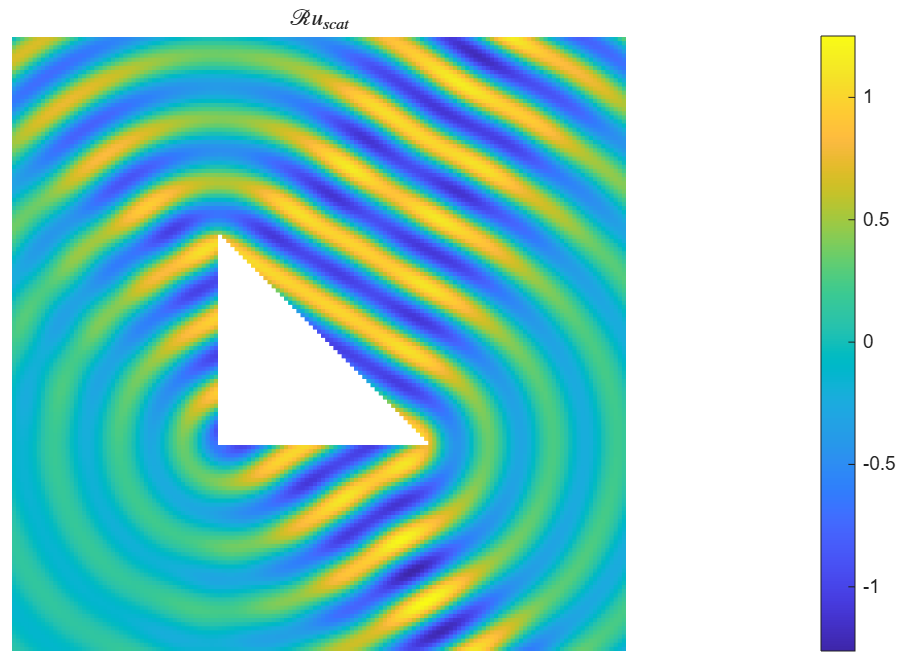
\includegraphics[width=\linewidth]{figures/tri_real_scat.png}
    \end{subfigure}
    \hfill
    \begin{subfigure}{0.45\textwidth}
        \centering
        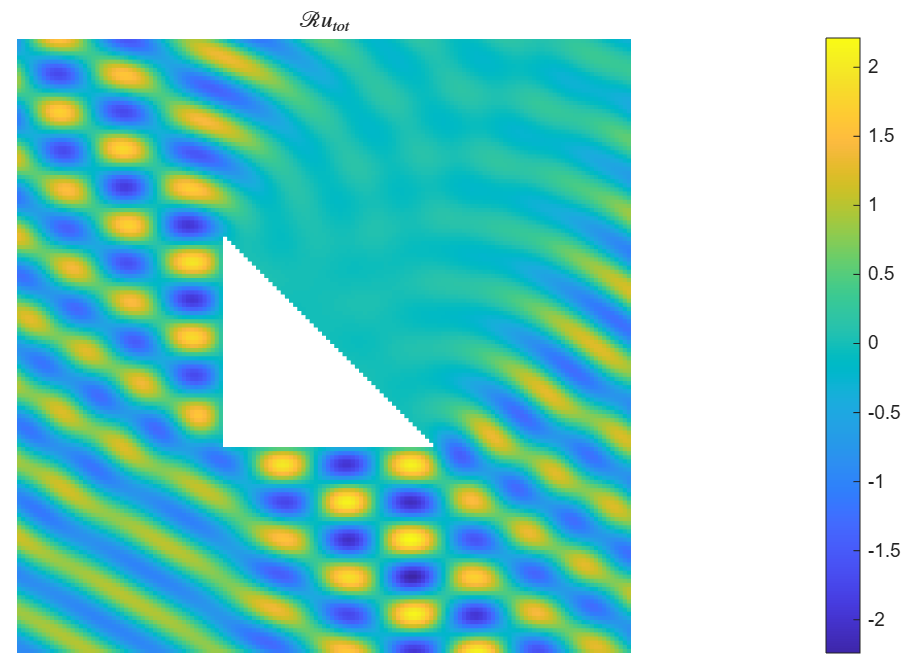
\includegraphics[width=\linewidth]{figures/tri_real_tot.png}
    \end{subfigure}

    \vspace{0.5cm}

    \begin{subfigure}{0.45\textwidth}
        \centering
        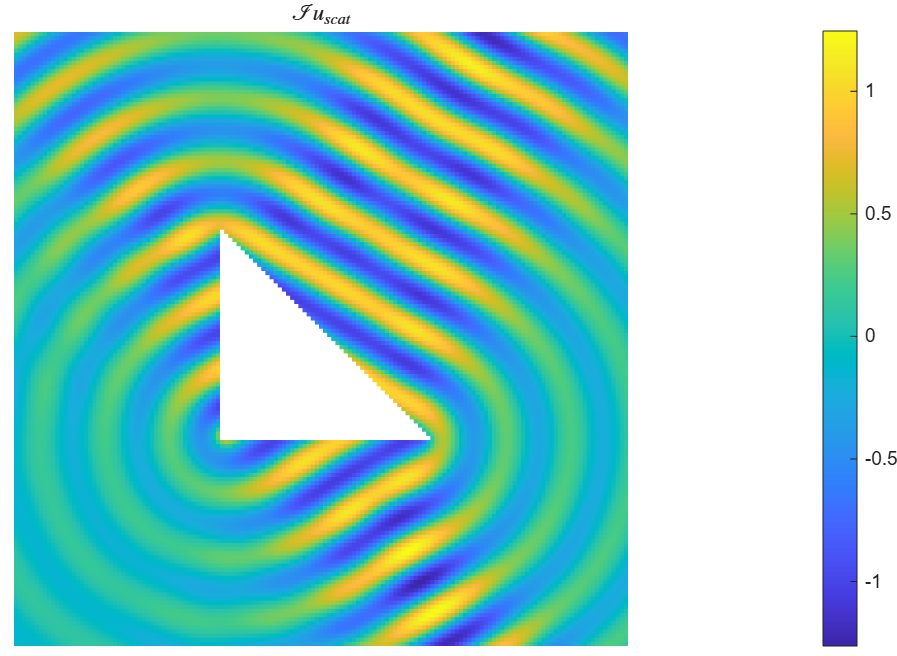
\includegraphics[width=\linewidth]{figures/tri_imag_scat.png}
    \end{subfigure}
    \hfill
    \begin{subfigure}{0.45\textwidth}
        \centering
        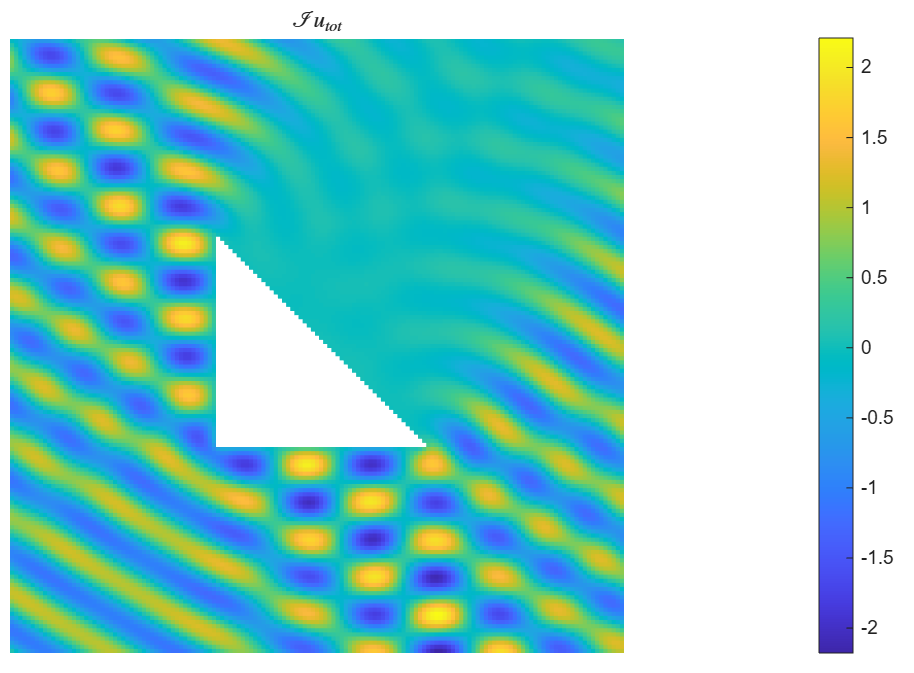
\includegraphics[width=\linewidth]{figures/tri_imag_tot.png}
    \end{subfigure}

    \vspace{0.5cm}

    \begin{subfigure}{0.45\textwidth}
        \centering
        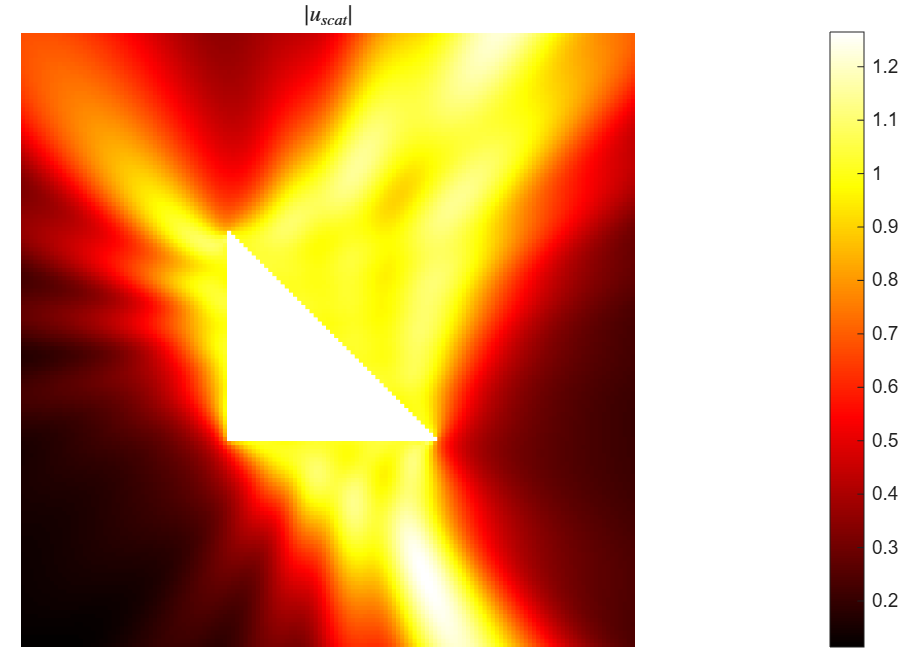
\includegraphics[width=\linewidth]{figures/tri_abs_scat.png}
        \caption{Campo scatterato}
    \end{subfigure}
    \hfill
    \begin{subfigure}{0.45\textwidth}
        \centering
        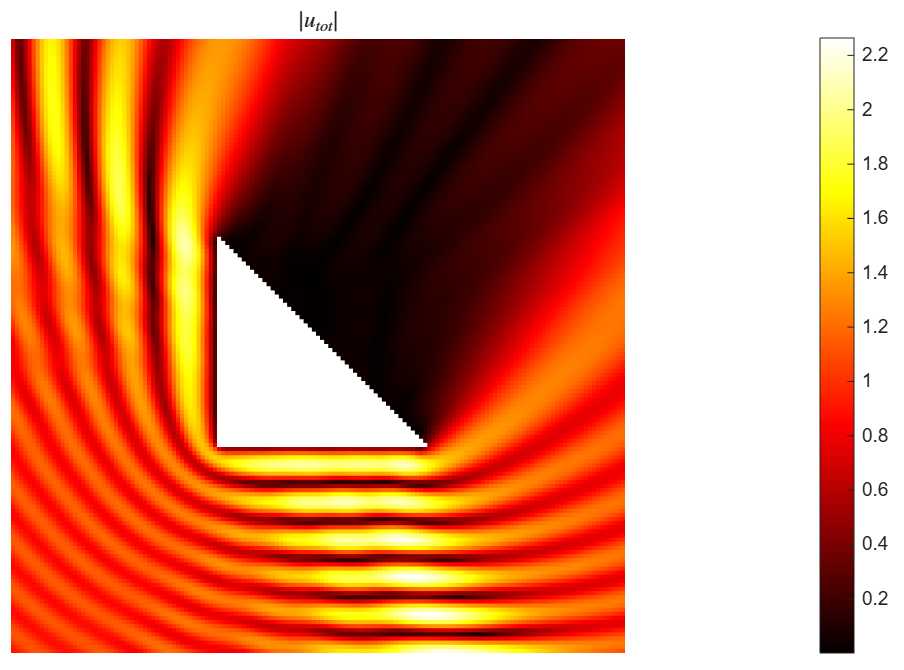
\includegraphics[width=\linewidth]{figures/tri_abs_tot.png}
        \caption{Campo totale}
    \end{subfigure}

    \caption{Campo scatterato (colonna sinistra) e campo totale (colonna destra) con onda piana incidente proveniente da $\theta = \frac{\pi}{3}$: parte reale, immaginaria e modulo.}
    \label{fig:tri_scattered_total}
\end{figure}

\subsection{Studio errore}
\label{subsec:studio errore}
Studiamo il comportamento dell'errore nel caso in cui $\Gamma$ sia un poligono, osservando come varia la soluzione numerica al raffinare della discretizzazione di $\Gamma$. \\
Consideriamo due tipi di test. Nel primo caso abbiamo a disposizione una soluzione  molto accurata che viene usata direttamente come riferimento per il calcolo dell'errore. Nel secondo caso, invece, la soluzione di riferimento viene approssimata con il metodo BEM stesso usando una discretizzazione molto fine.\\
Nella Figura \ref{fig:errMPSpack} viene riportato il grafico di convergenza per il metodo BEM a collocazione con funzioni di base costanti a tratti applicato allo scattering di un'onda piana da parte di un ostacolo quadrato $(0.5 \,,0.5 )^2$. Come soluzione di riferimento $u^{Ref}$ si utilizza quella ottenuta tramite MPSpack (disponibile a \url{ https://github.com/ahbarnett/mpspack}). Il grafico mostra l'errore relativo sul campo scatterato, definito come:
\begin{equation}
\label{eq:errore normalizzato}
    \frac{\|u^N - u^{Ref}\|_{L^2(D)}}{\|u^{Ref}\|_{L^2(D)}},
\end{equation}
dove $u^N$ rappresenta l'approssimazione BEM della soluzione esatta $u^{scat}$. L'insieme $D$ è il quadrato $(0.5 \,,0.5 )^2$ a cui è stato sottratto il disco unitario $B_1(0)$ in modo da evitare problemi legati alla quasi-singolarità nell'applicazione della formula di rappresentazione. Osserviamo che l'errore converge definitivamente con ordine circa uguale a $\frac{4}{3}$, in accordo con la teoria. I tempi computazionali per ogni iterazione sono riportati nella Tabella \ref{tab:time_MPSpack}

\begin{figure}[htbp]
    \centering
    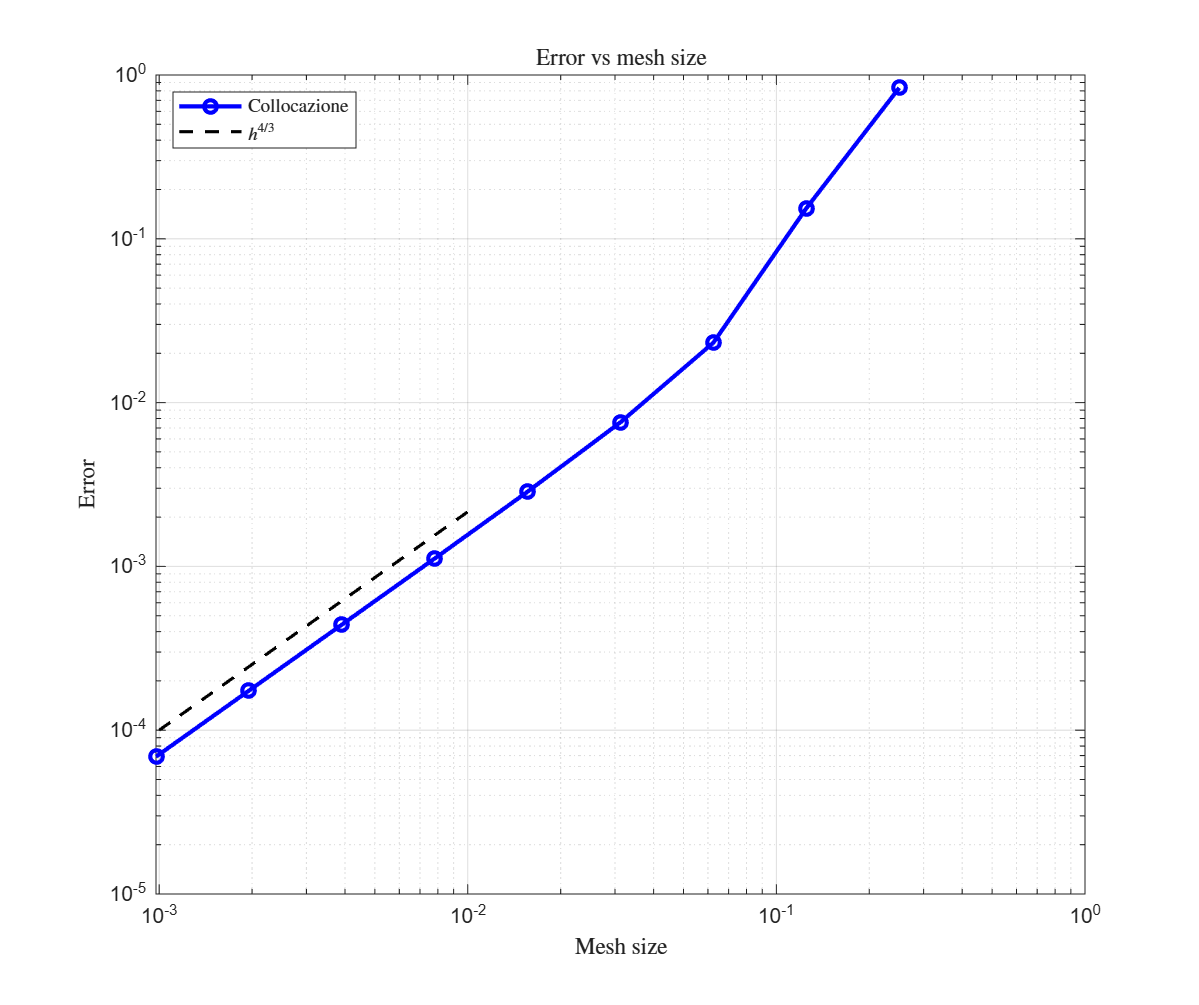
\includegraphics[width=0.5\linewidth]{figures/Err_mesh_MPSpack.png}
    \caption{Scattering di onda piana con angolo $\theta = -\pi/4$, numero d'onda $k=20$, mesh uniformi con $16, 32, \dots, 4096$ elementi. Per l'approssimazione degli integrali sono stati usati 5 nodi di Gauss per le entrate fuori dalla diagonale della matrice del sistema e per la formula di rappresentazione, e 30 nodi di Gauss per le entrate sulla diagonale della matrice.}
    \label{fig:errMPSpack}
\end{figure}

Consideriamo ora il caso in cui la soluzione di riferimento $u^{Ref}$ sia ottenuta a partire dallo stesso metodo BEM, ma con un numero di gradi di libertà molto elevato e guardiamo il comportamento dell'errore commesso da soluzioni ottenute con un numero di gradi di libertà progressivamente inferiore. I risultati ottenuti sono mostrati in Figura \ref{fig:err poligono}. in cui sono stati considerati gli stessi parametri del problema precedente e in cui viene mostrato l'errore definito dall'equazione \ref{eq:errore normalizzato}. Per calcolare la soluzione di riferimento sono stati utilizzati $N^{Ref}=4096$ gradi di libertà, mentre per le altre soluzioni sono stati usati $N=16, \dots, 2048$ gradi di libertà. Confrontando Figura \ref{fig:err poligono} con la Figura \ref{fig:errMPSpack} si può osservare che i due grafici sono qualitativamente simili. Sottolineiamo che dal semplice confronto dei due plot non si può dedurre che la soluzione di riferimento ottenuta con MPSpack sia migliore o peggiore di quella ottenuta con il metodo BEM con $4096$ gradi di libertà.
\begin{figure}
    \centering
    
\includegraphics[width=0.5\linewidth]{figures/Err_mesh_poly.png}
    \caption{numero d'onda $k=20$, angolo onda incidente $\theta=-\pi/4$; $ 4096$ gradi di libertà per la soluzione di riferimento, $N=16, \dots, 2048$ gradi di libertà per altre soluzioni; ostacolo $(0.5 \,,0.5 )^2$.}
    \label{fig:err poligono}
\end{figure}

Possiamo inoltre studiare il comportamento dell'errore di approssimazione della densità $\psi$ usata nella formula di rappresentazione calcolata numericamente attraverso la risoluzione dell'equazione integrale \ref{eq:bie}. Dal momento che non è necessario usare la formula di rappresentazione per calcolare $u^{scat}$ tramite il \textit{single layer potential} come mostrato nell'equazione \ref{eq:single_layer}, possiamo risparmiare molto tempo computazionale. Similmente a quanto accadeva prima, anche in questo caso la soluzione di riferimento $\psi^{Ref}$ è calcolata usando una mesh molto fine. Dal momento che la lunghezza del vettore $\psi$ coincide con il numero di gradi di libertà del problema, bisogna porre particolare attenzione sia alla scelta del numero di gradi di libertà, sia dell'ostacolo delimitato dal poligono $\Gamma$. \\
La densità di riferimento è stata calcolata con $N^{Ref}=2^{12}$ gradi di libertà, mentre le diverse approssimazioni hanno usato $N=2^4, \dots, 2^{11}$ gradi di libertà. In questo modo, per confrontare ad esempio la $\psi$ calcolata con $N=2^{11}$ con quella di riferimento era sufficiente ripetere ciascun suo valore una volta, seguendo lo schema $1^\circ, 1^\circ, 2^\circ, 2^\circ, \dots $, mantenendo così l'allineamento con $\psi^{Ref}$. \\
Come accennato in precedenza, è importante che il numero di gradi di libertà passati come input alla funzione che calcola $\psi$ coincida con quelli poi effettivamente usati dopo che è stato deciso in che modo distribuirli sui diversi lati del poligono. Infatti può capitare che tale numero aumenti lievemente nel caso in cui abbia poligoni non regolari oppure nel caso in cui il numero di gradi di libertà non sia un multiplo del numero di lati. Per questa ragione abbiamo considerato come ostacolo il quadrato $(-0.5, 0.5)^2$. I risultati di questo test sono mostrati nella Figura \ref{fig:psi err} in cui viene considerato l'errore descritto nell'equazione \ref{eq:errore normalizzato} ponendo $\psi$ in luogo di $u$.


\begin{figure}
    \centering
    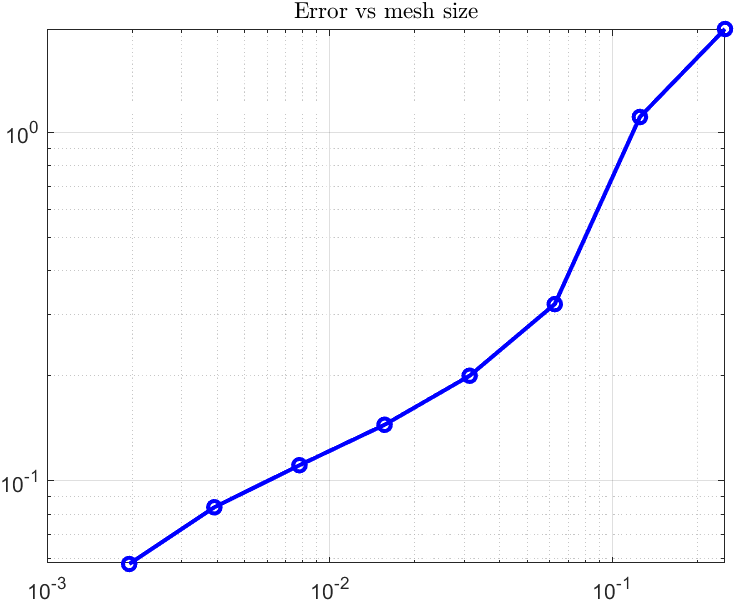
\includegraphics[width=0.5\linewidth]{figures/psi_err_vs_mesh.png}
    \caption{Grafico convergenza $\psi$ con $N^{Ref}=4096$, $N=16, \dots, 2048,$} ostacolo $(-0.5, 0.5)^2$, angolo di incidenza $\theta = -\pi/4$, numero d'onda $k=20$. 
    \label{fig:psi err}
\end{figure}



\newpage 
\section{Estensioni}
\label{sec:estensioni}
In questa sezione vengono riportate alcune estensioni del metodo di BEM descritto nella sezione \ref{sec:BEM_base}. Inoltre vengono descritti alcuni test effettuati per studiare la convergenza del metodo.
\subsection{Ostacolo curvilineo}
\label{subsec:ostacolo curvilineo}
Studiamo il caso in cui l'ostacolo non sia un poligono, ma presenti un bordo curvilineo (che indichiamo sempre con $\Gamma$) e di cui sia disponibile una rappresentazione parametrica. Rispetto al caso di base, la principale accortezza da avere riguarda la corretta collocazione dei nodi di quadratura, i quali devono appartenere al bordo $\Gamma$. Bisogna inoltre prestare attenzione al riscalamento dei nodi e pesi di quadratura che vengono utilizzati nell'approssimazione degli integrali che compaiono sia nell'assemblaggio della matrice del sistema, sia nella formula di rappresentazione. \\
I test numerici sono stati effettuati in due configurazioni geometriche distinte. In primo luogo si considera il caso della circonferenza, per la quale è possibile ottenere una soluzione di riferimento in modo analitico, permettendo quindi un'analisi più diretta del metodo al variare del numero di gradi di libertà del problema. Successivamente è stata considerata considerato un ostacolo \textit{kite} la cui rappresentazione parametrica è
\begin{equation}
\label{eq:parametrizzazione kite}
    \textbf{X}(t) = (\cos t + 0.65 (\cos 2t - 1), 1.5\sin t). 
\end{equation}
In questo caso, per studiare il comportamento dell'errore di approssimazione è stata preventivamente calcolata una soluzione di riferimento con un elevato numero di gradi di libertà ed abbiamo valutato l'errore commesso da soluzioni progressivamente meno fini. \\
Consideriamo in primo luogo una circonferenza di raggio $R$ centrata nell'origine ed un'onda piana con angolo di incidenza $\theta$. In questo caso è possibile sfruttare la semplice geometria dell'ostacolo per calcolare una soluzione di riferimento in modo analitico. Passando alle coordinate polari, possiamo individuare un generico punto $x \in \mathbb{C}$ tramite $x=r\cos \phi +ir\sin \phi$. Se indichiamo con $d=\exp(i\theta)$ il versore che descrive la direzione dell'onda incidente, allora si ha che $d = \cos \theta +i\sin\theta$. Usando la formula di espansione di Jacobi-Anger per le onde piane si ha
\begin{equation}
\label{eq:espansione campo inc}
    u^{inc}(\textbf{x})=\exp(ikd\cdot \textbf{x})=\exp(ikr\cos(\phi-\theta))= \sum_{l \in \mathbb{Z}}i^l\,J_l(kr)\, \exp(il(\phi -\theta)).
\end{equation}
L'onda scatterata viene rappresentata nella base delle funzioni di Hankel. In particolare consideriamo solo le $H_l^{(1)}$, in quanto la soluzione scatterata deve soddisfare la condizione di essere uscente. Quindi si ha 
\begin{equation*}
    u^{scat}(r, \phi)=\sum_{l \in \mathbb{Z}} A_l H_l^{(1)}(kr)\exp(il\phi).
\end{equation*}
Imponendo la condizione sound-soft studiata nel problema \ref{eq:edp} si ha
\begin{equation}
    \label{eq:coeff campo scat}
\begin{aligned}
    u^{tot}(R, \phi)=0 &\implies \sum_{l \in \mathbb{Z}}A_lH_l^{(1)}(kR)\exp(il\phi)=-\sum_{l \in \mathbb{Z}}i^l J_l(kR)\exp(il(\phi-\theta)) \\
    &\implies A_l=-i^l \frac{J_l(kR)}{H_l^{(1)}(kR)}e^{-il\theta} \\
    & \implies u^{scat}(r, \phi)=-\sum_{l \in \mathbb{Z}}i^l \frac{J_l(kR)}{H_l^{(1)}(kR)}H_l^{(1)}(kr)\exp(il\phi)\exp(-il\theta)
\end{aligned}
\end{equation}
Nei test che sono stati effettuati ho considerato una mesh $Z=x +iy$ nel piano complesso. In questa situazione, l'espressione del campo scattato può essere riscritta come
\begin{equation}
\label{eq:riscrittura campo scatterato}
\begin{aligned}
    &Z = r\exp(i\phi), \quad d=\exp(i\theta) \implies \left(\frac{Z}{d|Z|}\right)^l=\exp(il\phi)\exp(-il\theta) \\\\
    &u^{scat}(Z) = -\sum_{l \in \mathbb{Z}}i^l \frac{J_l(kR)}{H_l^{(1)}(kR)}H_l^{(1)}(kr) \left(\frac{Z}{d|Z|}\right)^l
\end{aligned}
\end{equation}
Nei test effettuati ho considerato una circonferenza di raggio $R=1$, un'onda incidente di angolo $\theta = \pi$ e numero d'onda $k=20$. 
Osserviamo che nel calcolo del campo scatterato di riferimento la somma su $l \in \mathbb{Z}$ deve essere troncata ad un valore $l_{max}$. Nella Figura \ref{fig:coeff circonferenza} ho riportato i moduli dei coefficienti del campo scatterato al variare di $k$ e $R$. Da tali grafici possiamo dedurre che sommatoria che definisce il campo scatterato può essere troncata ad un valore di poco superiore a $kR$. 

\begin{figure}[htbp]
\centering

\begin{subfigure}{0.45\textwidth}
    \centering
    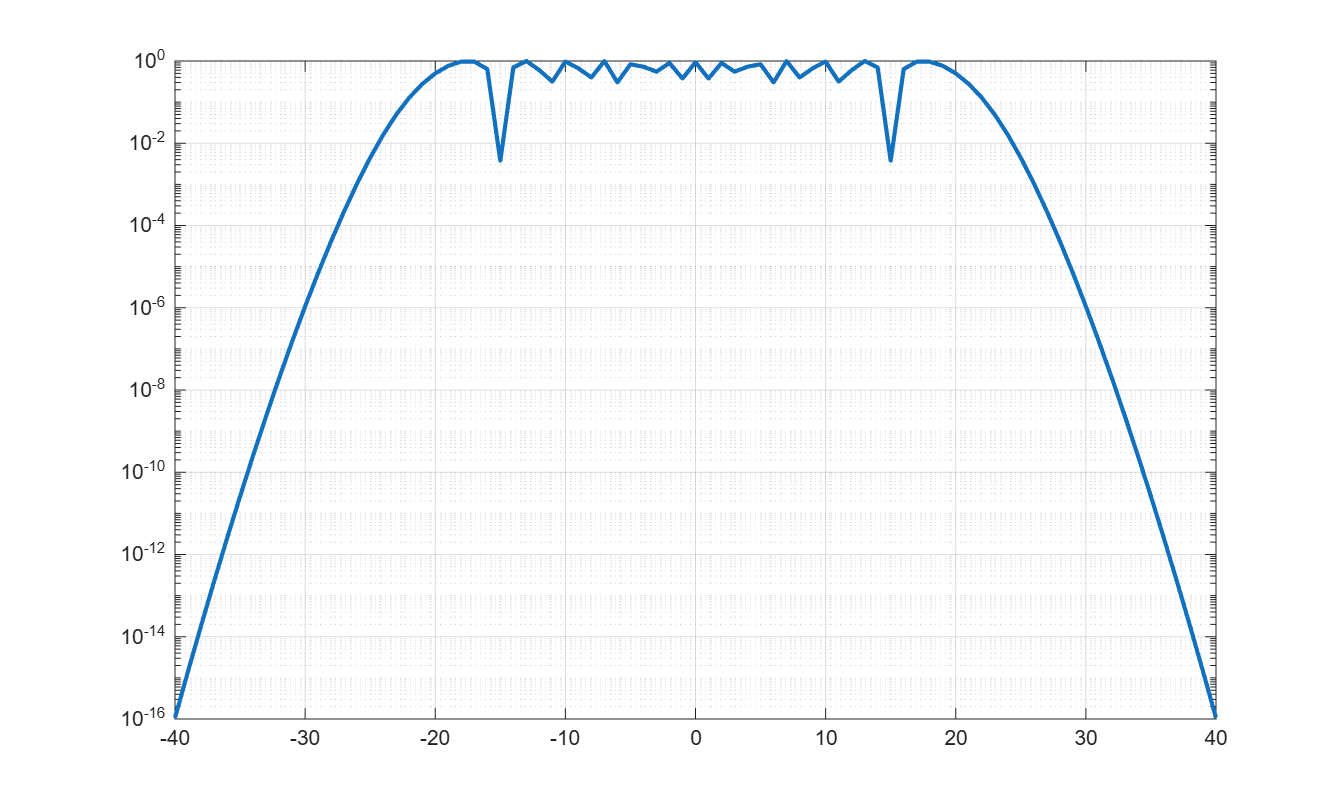
\includegraphics[width=\textwidth]{figures/coeff_R1_k20.png}
    \caption{$R=1, k=20$}
\end{subfigure}
\hfill
\begin{subfigure}{0.45\textwidth}
    \centering
    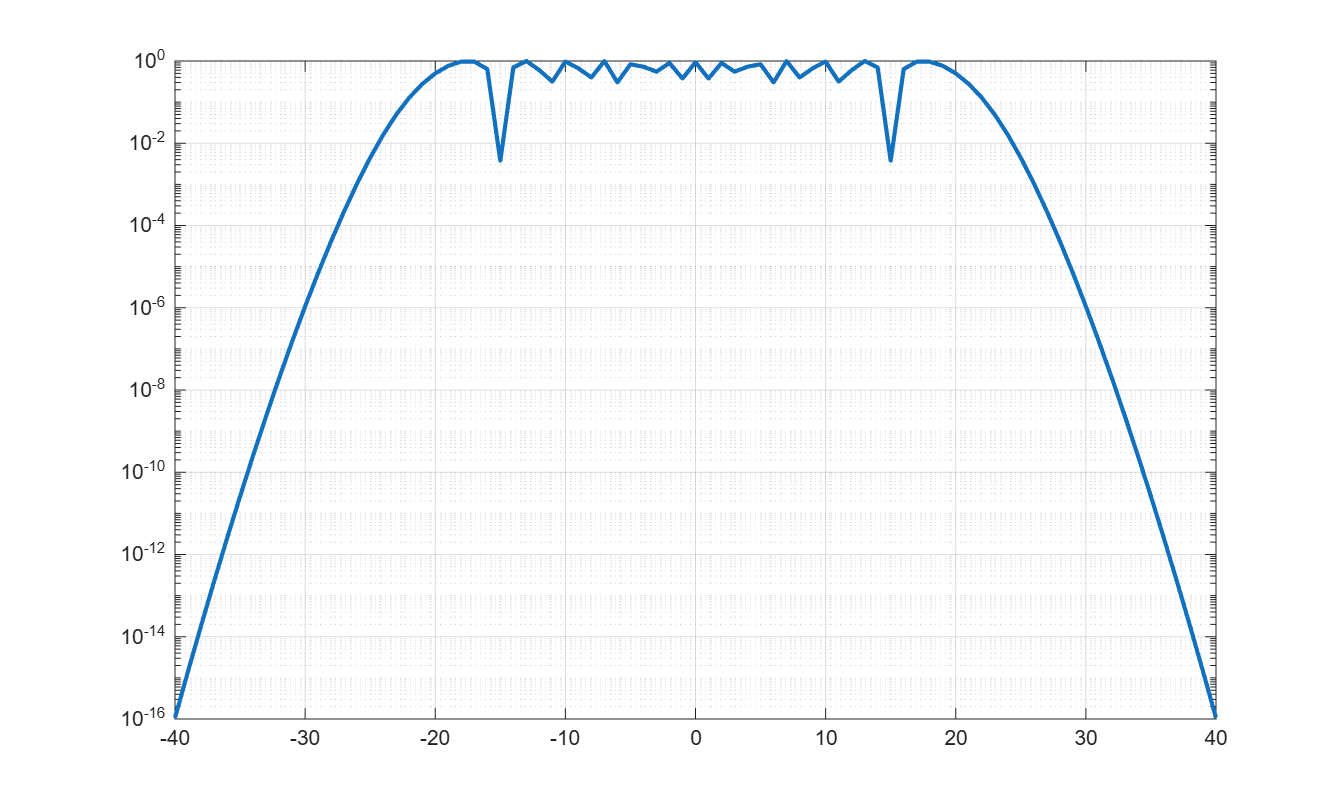
\includegraphics[width=\textwidth]{figures/coeff_R4_k5.png}
    \caption{$R=4, k=5$}
\end{subfigure}

\vspace{0.5cm}

\begin{subfigure}{0.45\textwidth}
    \centering
    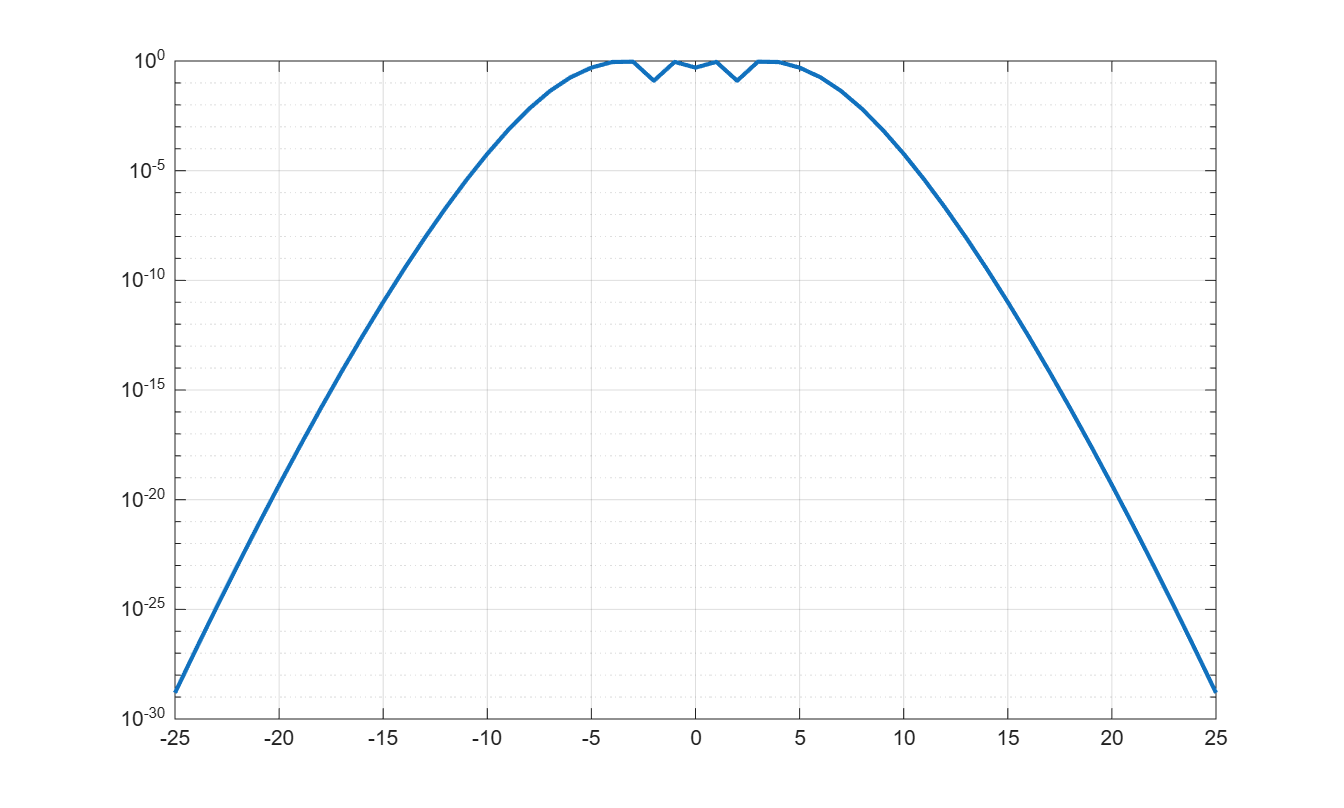
\includegraphics[width=\textwidth]{figures/coeff_R1_k5.png}
    \caption{$R=1, k=5$}
\end{subfigure}
\hfill
\begin{subfigure}{0.45\textwidth}
    \centering
    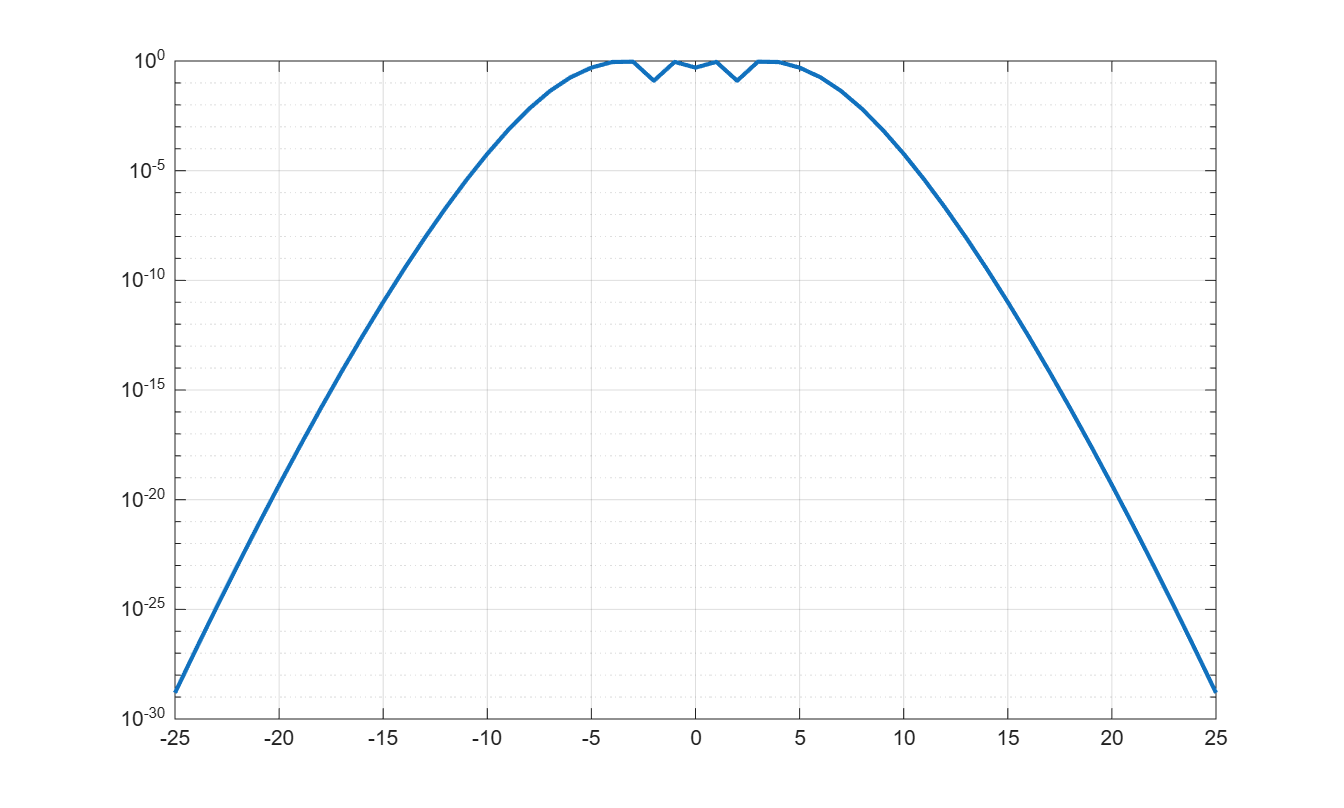
\includegraphics[width=\textwidth]{figures/coeff_R5_k1.png}
    \caption{$R=5, k=1$}
\end{subfigure}

\caption{Modulo dei coefficienti del campo scatterato per una circonferenza di raggio R e numero d'onda k.}
\label{fig:coeff circonferenza}
\end{figure}

Nella Figura \ref{fig:BEM circonferenza} vengono riportati i plot del campo scatterato e di quello totale. Similmente a quanto accadeva nella Figura \ref{fig:tri_scattered_total}, anche in questo caso si può vedere come il campo totale si annulli nella direzione di provenienza dell'onda incidente 

\begin{figure}[htbp]
    \centering

    \begin{subfigure}{0.45\textwidth}
        \centering
        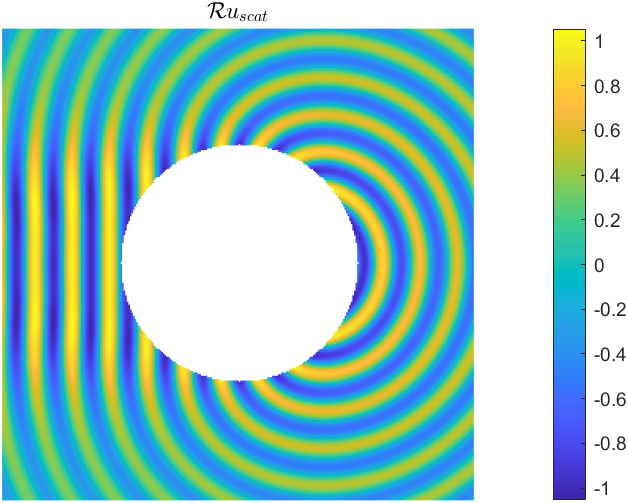
\includegraphics[width=\linewidth]{figures/circ_real_scat.png}
    \end{subfigure}
    \hfill
    \begin{subfigure}{0.45\textwidth}
        \centering
        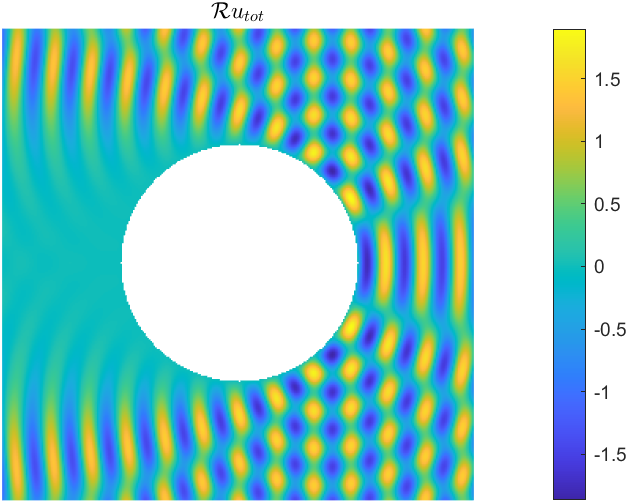
\includegraphics[width=\linewidth]{figures/circ_real_tot.png}
    \end{subfigure}

    \vspace{0.5cm}

    \begin{subfigure}{0.45\textwidth}
        \centering
        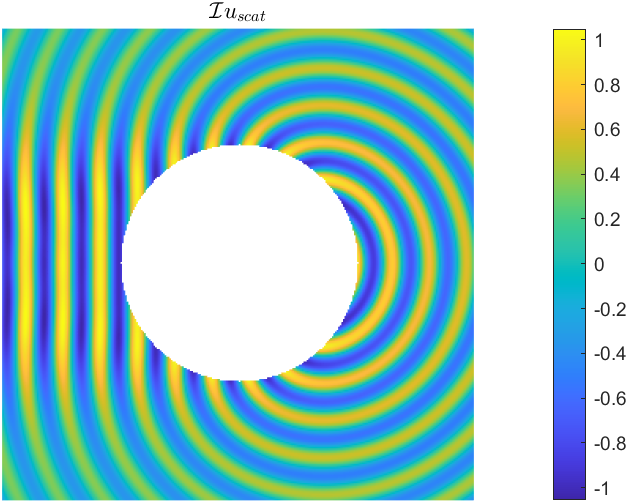
\includegraphics[width=\linewidth]{figures/circ_imag_scat.png}
    \end{subfigure}
    \hfill
    \begin{subfigure}{0.45\textwidth}
        \centering
        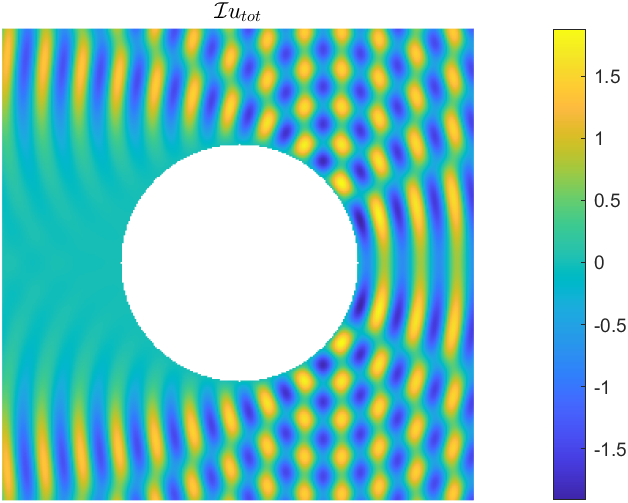
\includegraphics[width=\linewidth]{figures/circ_imag_tot.png}
    \end{subfigure}

    \vspace{0.5cm}

    \begin{subfigure}{0.45\textwidth}
        \centering
        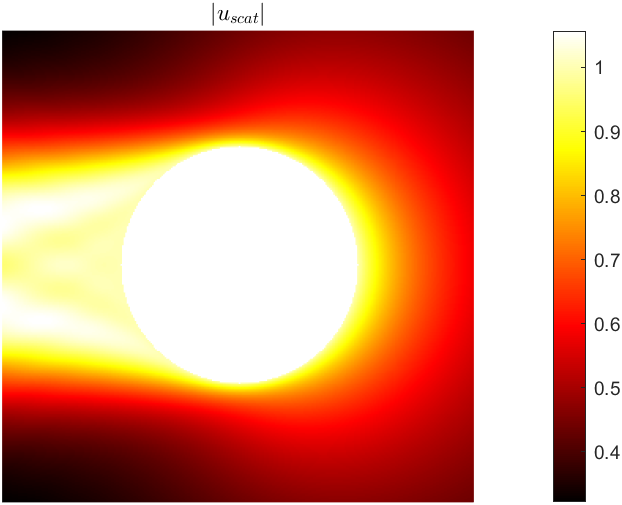
\includegraphics[width=\linewidth]{figures/circ_abs_scat.png}
        \caption{Campo scatterato}
    \end{subfigure}
    \hfill
    \begin{subfigure}{0.45\textwidth}
        \centering
        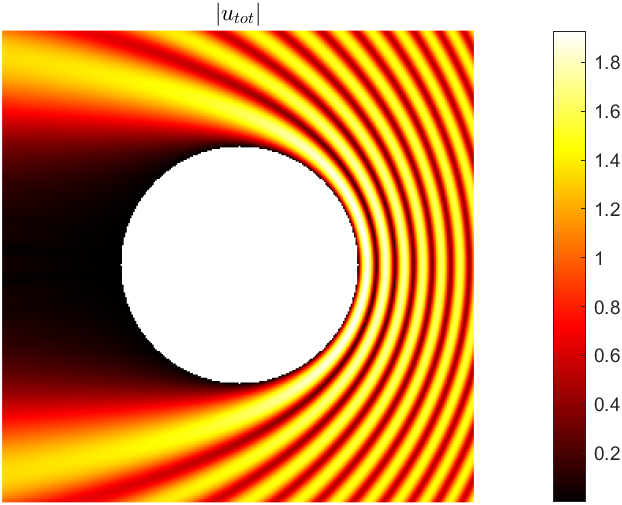
\includegraphics[width=\linewidth]{figures/circ_abs_tot.png}
        \caption{Campo totale}
    \end{subfigure}

    \caption{Campo scatterato (colonna sinistra) e campo totale (colonna destra) con onda piana incidente proveniente da $\theta = \pi$: parte reale, immaginaria e modulo.}
    \label{fig:BEM circonferenza}
\end{figure}

Nella Figura \ref{fig:BEM kite} vengono riportati i plot del campo scatterato e del campo totale nel caso in cui il bordo dell'ostacolo sia parametrizzato dall'equazione \ref{eq:parametrizzazione kite}.

\begin{figure}[htbp]
    \centering

    \begin{subfigure}{0.45\textwidth}
        \centering
        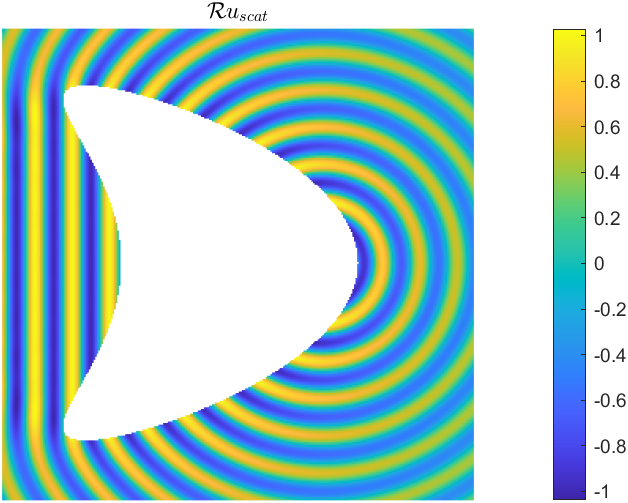
\includegraphics[width=\linewidth]{figures/kite_real_scat.png}
    \end{subfigure}
    \hfill
    \begin{subfigure}{0.45\textwidth}
        \centering
        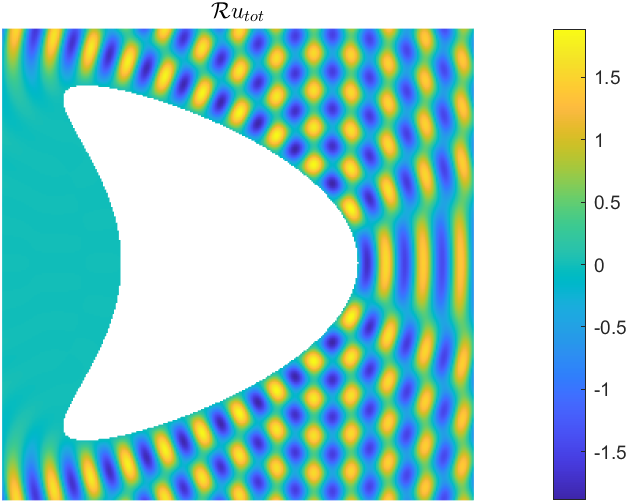
\includegraphics[width=\linewidth]{figures/kite_real_tot.png}
    \end{subfigure}

    \vspace{0.5cm}

    \begin{subfigure}{0.45\textwidth}
        \centering
        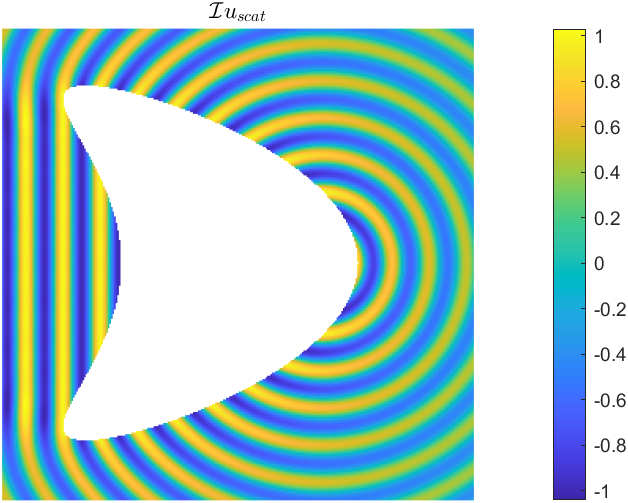
\includegraphics[width=\linewidth]{figures/kite_imag_scat.png}
    \end{subfigure}
    \hfill
    \begin{subfigure}{0.45\textwidth}
        \centering
        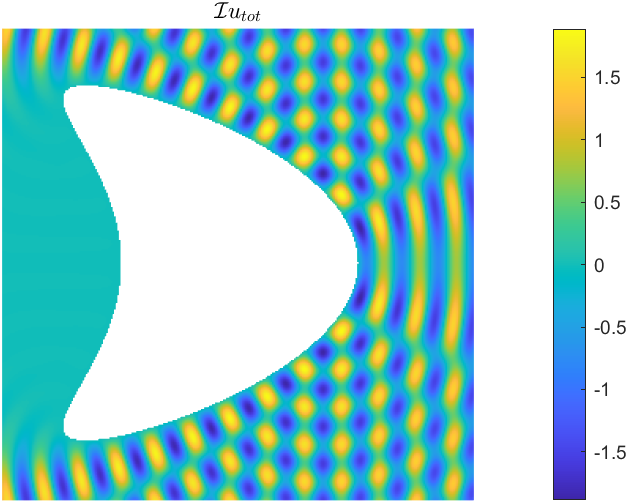
\includegraphics[width=\linewidth]{figures/kite_imag_tot.png}
    \end{subfigure}

    \vspace{0.5cm}

    \begin{subfigure}{0.45\textwidth}
        \centering
        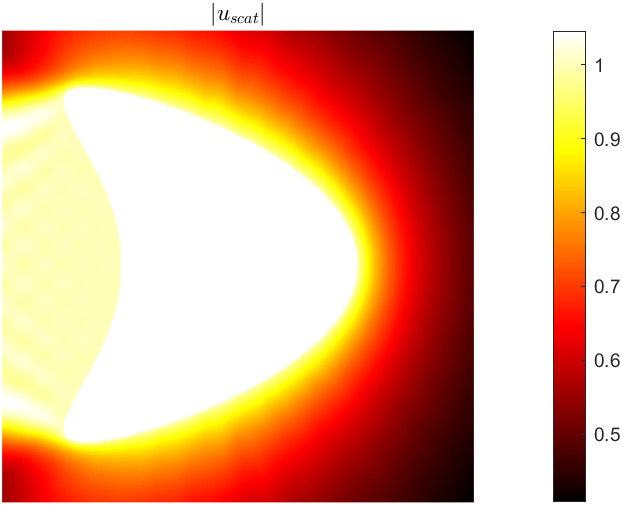
\includegraphics[width=\linewidth]{figures/kite_abs_scat.png}
        \caption{Campo scatterato}
    \end{subfigure}
    \hfill
    \begin{subfigure}{0.45\textwidth}
        \centering
        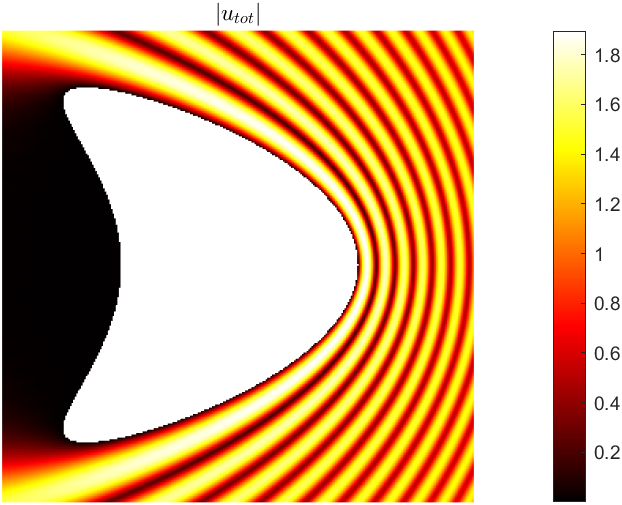
\includegraphics[width=\linewidth]{figures/kite_abs_tot.png}
        \caption{Campo totale}
    \end{subfigure}

    \caption{Campo scatterato (colonna sinistra) e campo totale (colonna destra) con onda piana incidente proveniente da $\theta = \pi$: parte reale, immaginaria e modulo.}
    \label{fig:BEM kite}
\end{figure}
\newpage
\subsection{Proximity resonance}
\label{subsec:proximity resonance}
In questa estensione del metodo BEM si considera il caso in cui l'onda incidente abbia una sorgente in prossimità dell'ostacolo $\Gamma$. L'obiettivo è studiare il campo totale al variare della distanza tra sorgente e ostacolo. In particolare, nella Figura \ref{fig:proximity resonance} vengono mostrati i risultati numerici nel caso in cui:
\begin{itemize}
    \item $\Gamma$ ostacolo sound-soft di vertici $V_1 = (0, 1/2), V_2=(-1/2, 0), V_3=(0, -1/2)$;
    \item $u^{inc}(\textbf{x}) = \Phi_k(\textbf{x}, \textbf{y})$;
    \item $k=20$ numero d'onda;
    \item $\lambda= \frac{2\pi}{k}$ lunghezza d'onda; 
    \item $d \in \{\frac{\lambda}{4}, \frac{\lambda}{2}, \frac{3\lambda}{4}\}$ distanza tra la sorgente di $u^{inc}$ e il lato $\overline{V_1 V_3}$ di $\Gamma$; 
\end{itemize}

Dal momento che stiamo considerando un ostacolo sound-soft si ha un'inversione di fase di $\pi$ al momento della riflessione.
I risultati numerici mostrano un comportamento molto diverso nei tre casi analizzati. \\
Quando $d= \frac{\lambda}{4}$ (Figura \ref{fig:proximity resonance}(a)), si ha che il cammino totale percorso è pari a $2d = \frac{\lambda}{2}$. Quindi lo sfasamento accumulato lungo questo percorso è dato da $2kd = k \frac{\lambda}{2} = k \frac{2\pi}{2k} = \pi $. A questo sfasamento si deve aggiungere $\pi$ per considerare l'inversione di fase. Il risultato finale è un ritorno in fase dell'onda scatterata.\\
Nel caso in cui $d= \frac{\lambda}{2}$ (Figura \ref{fig:proximity resonance}(b)) si ha il fenomeno opposto rispetto a quello descritto sopra. Infatti in questo caso nel tragitto di andata e ritorno dell'onda incidente copre una distanza pari alla lunghezza d'onda $\lambda$; tuttavia per l'inversione di fase che deriva dall'ostacolo sound-soft porta l'onda scatterata ad avere una fase opposta. Dunque si crea interferenza distruttiva. \\
Nel caso in cui $d= \frac{3\lambda}{4}$ si ha che $2d = \frac{3\lambda}{2}$ e dunque lo sfasamento accumulato lungo il percorso è pari a $2kd=\frac{6k\pi}{2k}=3\pi$ a cui si devo sommare $\pi$ per la riflessione. Abbiamo dunque che lo sfasamento totale pari ad un multiplo intero di $2\pi$ e quindi l'onda scatterata torna alla sorgente perfettamente in fase con le nuove onde che la sorgente stessa sta emettendo in quel momento. Si ha dunque interferenza costruttiva lungo il segmento passante per la sorgente e ortogonale al lato dell'ostacolo. Le zone più scure che si possono vedere convergere verso la sorgente nella Figura \ref{fig:proximity resonance}(c) indicano punti dello spazio in cui si ha interferenza distruttiva. Consideriamo un generico punto $P(\textbf{x})$ nel dominio:
\begin{itemize}
    \item sia $r$ la distanza euclidea tra la sorgente e il punto $P$;
    \item sia $r_{rifl}$ il cammino totale che compie l'onda per andare dalla sorgente al lato dell'ostacolo e poi raggiungere il punto $P$
\end{itemize}
La condizione per cui il campo totale si annulli in $P$ richiede che la differenza di fase tra l'onda riflessa e quella diretta sia un multiplo dispari di $\pi$, ovvero deve essere che
\begin{equation*}
    \Delta\phi(P) = k(r_{rifl} -r)+ \pi = (2n+1)\pi \implies k(r_{rifl} -r)= 2n\pi
\end{equation*}
per qualche $n \in \mathbb{N}$. In questo esempio, l'unico valore ammissibile è $n = 1 $ dal momento che $r_{rifl} - r\leq 2d$ e quindi $2n\pi \leq k\cdot 2d = 3\pi$. Dunque la condizione di interferenza distruttiva in $P$ si può tradurre in
\begin{equation*}
    r_{rifl} - r = \frac{2\pi}{k}=\lambda,
\end{equation*}
che è l'espressione di un'iperbole.  \\
Osserviamo inoltre che questo comportamento non si ha nel primo caso, in cui $d=\frac{\lambda}{4}$ dal momento che $r_{rifl}-r \leq 2d= \frac{\lambda}{2}$. Poiché questo valore è inferiore alla lunghezza d'onda $\lambda$, la condizione $r_{rifl}-r=\lambda$ non può mai essere soddisfatta in nessun punto del dominio. Invece, nel caso $d=\frac{3\lambda}{4}$ si ha che il cammino massimo di riflessione è $2d = \frac{3\lambda}{2}\geq \lambda$, dunque esistono delle traiettorie nel dominio che verificano quest'uguaglianza.
Per ulteriori dettagli si può fare riferimento a \cite{ProxRes}, p. 193.
\begin{figure}[htbp]
    \centering
    
    \begin{subfigure}{0.32\textwidth}
        \centering
        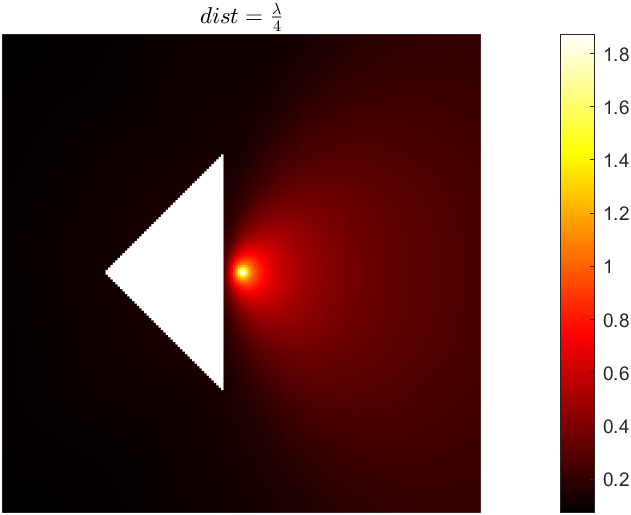
\includegraphics[width=\textwidth]{figures/ProximityResonance/lambda4.png}
        \caption{$d = \lambda/4$}
    \end{subfigure}
    \hfill
    \begin{subfigure}{0.32\textwidth}
        \centering
        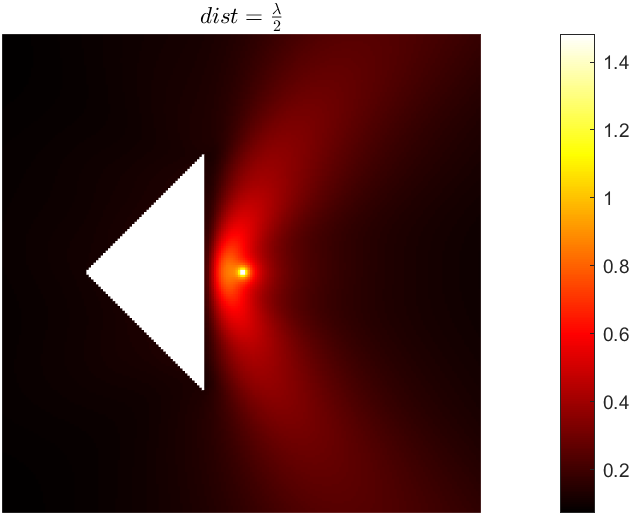
\includegraphics[width=\textwidth]{figures/ProximityResonance/lambda2.png}
        \caption{$d = \lambda/2$}
    \end{subfigure}
    \hfill
    \begin{subfigure}{0.32\textwidth}
        \centering
        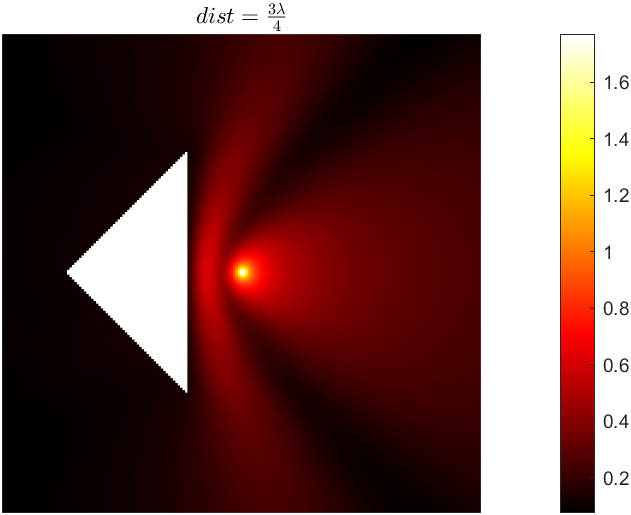
\includegraphics[width=\textwidth]{figures/ProximityResonance/3lambda4.png}
        \caption{$d = 3\lambda/4$}
    \end{subfigure}

    \caption{Confronto proximity resonance al variare della distanza $d$ dal lato dell'ostacolo $\Gamma$}
    \label{fig:proximity resonance}
\end{figure}
\newpage
\subsection{Altre estensioni}
\label{subsec:altre estensioni}
In questa sezione sono riportate altre estensioni minori del codice BEM di base descritto in precedenza. In particolare nella Figura \ref{fig:soluzione fondamentale contro poligono} vengono riportati i grafici dei campi incidente, scatterato e totale nel caso in cui il campo incidente sia costituito dalla soluzione fondamentale 
\begin{equation*}
    \Phi_k(x, y) = \frac{i}{4}H_0^{(1)}(k|x-y|), \quad x, y \in \mathbb{C}.
\end{equation*}
In particolare ho usato $k=20, y = 0.5+0.5i$, mentre l'ostacolo è costituito dal triangolo di vertici $(-0.5, 0.5); (-0.5, -0.5); (0.5, -0.5)$.
Con gli stessi parametri, nella Figura \ref{fig:onda circolare contro poligono} vengono mostrati i campi incidente, scatterato e totale nel caso in cui il campo incidente sia $H_3^{(1)}(k|x-x_0|)e^{3i\theta}$ con $x_0 = (0.5, 0.5), k=20$.\\
In entrambi i casi le zone scure nella rappresentazione dei valori assoluti del campo totale possono essere spiegate con un ragionamento analogo a quanto visto nella sezione \ref{subsec:proximity resonance}.



\begin{figure}[htbp]
\centering

% riga 1
\begin{subfigure}{0.3\textwidth}
    
\includegraphics[width=\linewidth]{figures/fond_real_inc.png}
\end{subfigure}
\begin{subfigure}{0.3\textwidth}
    
\includegraphics[width=\linewidth]{figures/fond_imag_inc.png}
\end{subfigure}
\begin{subfigure}{0.3\textwidth}
    
\includegraphics[width=\linewidth]{figures/fond_abs_inc.png}
\end{subfigure}

\vspace{0.3cm}

% riga 2
\begin{subfigure}{0.3\textwidth}
    
\includegraphics[width=\linewidth]{figures/fond_real_scat.png}
\end{subfigure}
\begin{subfigure}{0.3\textwidth}
    
\includegraphics[width=\linewidth]{figures/fond_imag_scat.png}
\end{subfigure}
\begin{subfigure}{0.3\textwidth}
    
\includegraphics[width=\linewidth]{figures/fond_abs_scat.png}
\end{subfigure}

\vspace{0.3cm}

% riga 3
\begin{subfigure}{0.3\textwidth}
    
\includegraphics[width=\linewidth]{figures/fond_real_tot.png}
\end{subfigure}
\begin{subfigure}{0.3\textwidth}
    
\includegraphics[width=\linewidth]{figures/fond_imag_tot.png}
\end{subfigure}
\begin{subfigure}{0.3\textwidth}
    
\includegraphics[width=\linewidth]{figures/fond_abs_tot.png}
\end{subfigure}

\caption{Onda incidente è la soluzione fondamentale centrata in (0.5, 0.5) con $k=20$.\\
Lungo le righe: campo incidente, campo scatterato e campo totale. \\
Lungo le colonne: parte reale, parte immaginaria, modulo}
\label{fig:soluzione fondamentale contro poligono}

\end{figure}


\begin{figure}[htbp]
\centering

% riga 1
\begin{subfigure}{0.3\textwidth}
    
\includegraphics[width=\linewidth]{figures/onda_circ_real_inc.png}
\end{subfigure}
\begin{subfigure}{0.3\textwidth}
    
\includegraphics[width=\linewidth]{figures/onda_circ_imag_inc.png}
\end{subfigure}
\begin{subfigure}{0.3\textwidth}
    
\includegraphics[width=\linewidth]{figures/onda_circ_abs_inc.png}
\end{subfigure}

\vspace{0.3cm}

% riga 2
\begin{subfigure}{0.3\textwidth}
    
\includegraphics[width=\linewidth]{figures/onda_circ_real_scat.png}
\end{subfigure}
\begin{subfigure}{0.3\textwidth}
    
\includegraphics[width=\linewidth]{figures/onda_circ_imag_scat.png}
\end{subfigure}
\begin{subfigure}{0.3\textwidth}
    
\includegraphics[width=\linewidth]{figures/onda_circ_abs_scat.png}
\end{subfigure}

\vspace{0.3cm}

% riga 3
\begin{subfigure}{0.3\textwidth}
    
\includegraphics[width=\linewidth]{figures/onda_circ_real_tot.png}
\end{subfigure}
\begin{subfigure}{0.3\textwidth}
    
\includegraphics[width=\linewidth]{figures/onda_circ_imag_tot.png}
\end{subfigure}
\begin{subfigure}{0.3\textwidth}
    
\includegraphics[width=\linewidth]{figures/onda_circ_abs_tot.png}
\end{subfigure}

\caption{Il campo incidente è $H_3^{(1)}(k|x-x_0|)e^{3i\theta}$ con $x_0 = (0.5, 0.5), k=20$.\\
Lungo le righe: campo incidente, campo scatterato e campo totale. \\
Lungo le colonne: parte reale, parte immaginaria, modulo}
\label{fig:onda circolare contro poligono}

\end{figure}

\newpage
\section{Far Field Pattern}
In questa sezione estendiamo l'analisi del problema di scattering definito nell'equazione \ref{eq:edp}, focalizzandoci sul comportamento asintotico del campo scatterato $u^{scat}$ a grande distanza dall'ostacolo $\Gamma$. 

In generale, si può dimostrare (si veda, ad esempio, \cite{CK19}, eq. (3.109)) che ogni soluzione $u$ dell'equazione di Helmholtz che soddisfi la condizione di radiazione di Sommerfeld (SRC) ammette lo sviluppo asintotico:
\begin{equation}
	\label{eq:relazione u_scat e ffp}
	u(\textbf{x}) = \frac{e^{ikr}}{\sqrt{r}} \left( u_\infty (\hat{x}	) + \mathcal{O}\left(\frac{1}{r}\right) \right) \qquad \text{per } r = |\textbf{x}| \rightarrow +\infty.
\end{equation}
La funzione a valori complessi $u_\infty(\hat{x})$ prende il nome di \textit{Far Field Pattern} (FFP) ed è definita sulla circonferenza unitaria in termini del versore $\hat{x} = \frac{\textbf{x}}{|\textbf{x}|}$. Nel contesto bidimensionale, risulta naturale parametrizzare tale versore mediante l'angolo di osservazione $\theta \in [0, 2\pi)$, ponendo
\begin{equation*}
	\hat{x} = \begin{pmatrix} \cos\theta \\ \sin\theta \end{pmatrix}.
\end{equation*}
Nel caso in cui $\Gamma$ sia il bordo di un ostacolo limitato e aperto il cui complementare è un dominio illimitato di classe $C^2$ si ha che 
\begin{equation}
	\label{eq:ffp generale}
	u_\infty (\hat{x}) = \frac{1}{4\pi} \int_\Gamma \left\{\gamma^+u(\textbf{y})\partial_\textbf{n}^+ e^{-ik\hat{x} \cdot \textbf{y}} - \partial_\textbf{n}^+ u(\textbf{y}) e^{-ik\hat{x} \cdot \textbf{y}} \right\} ds(\textbf{y}),
\end{equation}
dove $\gamma^+, \partial_n^+$ sono rispettivamente gli operatori di traccia di Dirichlet e Neumann esterni  e $\textbf{n}$ è il versore normale uscente da $\Omega_-$.

\subsection{Far field per ostacoli poligonali}
Nel caso in cui l'ostacolo sia un poligono non è necessario calcolare esplicitamente la traccia e la derivata normale del campo scatterato per valutare l'equazione \ref{eq:ffp generale}. Dal momento che abbiamo costruito la soluzione $u^{scat}$ attraverso la formula di rappresentazione \ref{eq:single_layer}, possiamo ricavare il far field in modo più diretto, studiando il comportamento asintotico della soluzione fondamentale. \\
Per fare ciò, analizziamo prima di tutto il comportamento di $|\textbf{x}- \textbf{y}|$ con $|\textbf{x}| \rightarrow + \infty $ e $\textbf{y} \in \Gamma $. Sfruttando le proprietà del prodotto scalare, si ha
\begin{equation*}
	|\textbf{x}-\textbf{y}|^2 = |\textbf{x}|^2 - 2\textbf{x}\cdot \textbf{y} + |\textbf{y}|^2= |\textbf{x}| \sqrt{1- \frac{2\textbf{x}\cdot \textbf{y}}{|\textbf{x}|^2} + \frac{|\textbf{y}|^2}{|\textbf{x}|^2}}.
\end{equation*}
Dal momento che $|\textbf{x}|\rightarrow + \infty $ possiamo utilizzare lo sviluppo in serie di Taylor al primo ordine $\sqrt{1+t}= 1+\frac{1}{2}t + \mathcal{O}(t^2) \text{ per } t \rightarrow 0$. Applicandolo alla nostra espressione si ottiene:
\begin{equation*}
	|\textbf{x}-\textbf{y}| \approx |\textbf{x}| \left(1-\frac{\textbf{x}\cdot \textbf{y}}{|\textbf{x}|^2} + \mathcal{O}\left(\frac{1}{|\textbf{x}|^2}\right)\right) = |\textbf{x}|- \frac{\textbf{x}\cdot \textbf{y}}{|\textbf{x}|} + \mathcal{O}\left(\frac{1}{|\textbf{x}|}\right).
\end{equation*}
Sostituendo la definizione del versore $\hat{x} = \frac{\textbf{x}}{|\textbf{x}|} $ ricaviamo: 

\begin{equation}
	\label{eq:ffp con approssimazione distanza}
	|\textbf{x} - \textbf{y}| \approx |\textbf{x}| - \hat{x} \cdot \textbf{y} \quad \text{per } |\textbf{x}| \to \infty.
\end{equation}


Consideriamo ora la soluzione fondamentale $\Phi (\textbf{x}, \textbf{y})=\frac{i}{4}H_0^{(1)}(k|\textbf{x}-\textbf{y}|)$.\\
 Si può dimostrare che:
\begin{equation}
	\label{eq:soluzione fondamentale asintotica}
	H_0^{(1)}(z) \approx \sqrt{\frac{2}{\pi z}} e^{i(z-\pi/4)} \qquad \text{per } z \rightarrow + \infty.
\end{equation}

Ponendo $z= k|\textbf{x}-\textbf{y}|$ si ottiene

\begin{equation*}
	H_0^{(1)}(k|\textbf{x}-\textbf{y}|) \approx \sqrt{\frac{2}{\pi k|\textbf{x}-\textbf{y}|}} e^{i(k|\textbf{x}-\textbf{y}|-\pi/4)}.
\end{equation*}

Al denominatore abbiamo $\sqrt{|\textbf{x}-\textbf{y}|}$, dal momento che $|\textbf{x}|\rightarrow + \infty $, il termine $\hat{x}\cdot \textbf{y}$ è un numero limitato e quindi diventa infinitesimo rispetto a $|\textbf{x}|$. Dunque al denominatore possiamo semplicemente trascurare la $\textbf{y}$ e abbiamo
\begin{equation*}
	\sqrt{\frac{2}{\pi k |\textbf{x}-\textbf{y}|}} \approx \sqrt{\frac{2}{\pi k |\textbf{x}|}}.
\end{equation*}

Al numeratore abbiamo $e^{ik |\textbf{x}-\textbf{y}|}$, sostituendo l'approssimazione $|\textbf{x}-\textbf{y}| \approx |\textbf{x}| - \hat{x}\cdot \textbf{y}$ otteniamo:
\begin{equation*}
	e^{ik(|\textbf{x}| - \hat{x}\cdot \textbf{y})} = e^{ik|\textbf{x}|} e^{-ik\hat{x}\cdot \textbf{y}}.
\end{equation*}
Sostituendo le due approssimazioni nella funzione di Hankel asintotica otteniamo:
\begin{equation*}
	H_0^{(1)}(k|\textbf{x}-\textbf{y}|) \approx \sqrt{\frac{2}{\pi k |\textbf{x}|}}e^{ik|\textbf{x}|}e^{-ik \hat{x}\cdot \textbf{y}}e^{-i\pi/4}. 
\end{equation*}
Infine, l'approssimazione asintotica della soluzione fondamentale diventa
\begin{equation}
	\Phi(\textbf{x}, \textbf{y})= \frac{i}{4}H_0^{(1)}(k|\textbf{x}-\textbf{y}|) \approx \frac{e^{i\pi /4}}{\sqrt{8\pi k |\textbf{x}|}}e^{ik|\textbf{x}|}e^{-ik \hat{x}\cdot \textbf{y}}.
\end{equation}


Considerando l'equazione \ref{eq:relazione u_scat e ffp} e le diverse approssimazione che abbiamo discusso si ha che 
\begin{equation*}
	\begin{aligned}
		\frac{e^{ik|\textbf{x}|}}{\sqrt{|\textbf{x}|}} u_\infty(\hat{x}) \approx u^{scat}(\textbf{x}) &\approx \int_\Gamma \frac{e^{i\pi/4}}{\sqrt{8\pi k |\textbf{x}|}} e^{ik|\textbf{x}|}e^{-ik\hat{x}\cdot \textbf{y}} \psi(\textbf{y})ds(\textbf{y})\\
		&= \frac{e^{i\pi/4}}{\sqrt{8\pi k |\textbf{x}|}} e^{ik|\textbf{x}|} \int_\Gamma e^{-ik\hat{x}\cdot \textbf{y}} \psi(\textbf{y})ds(\textbf{y}).
	\end{aligned}
\end{equation*}

Ricavando l'espressione del far field $u_\infty$ si ottiene
\begin{equation}
	\label{eq:ffp poligono}
	u_\infty(\hat{x}) \approx \frac{e^{i\pi/4}}{\sqrt{8\pi k }}\int_\Gamma e^{-ik \hat{x}\cdot \textbf{y}}\psi(\textbf{y}) ds(\textbf{y}).
\end{equation}

Da un punto di vista computazionale, la formulazione integrale \ref{eq:ffp poligono} per calcolare il far field presenta un vantaggio significativo rispetto al campo scatterato $u^{scat}$. Per valutare quest'ultimo tramite il \textit{single layer potential} (eq. \ref{eq:single_layer}), infatti, è necessario integrale la soluzione fondamentale $\Phi_k(\textbf{x}, \textbf{y})$, la quale presenta una singolarità logaritmica quando il punto di osservazione $\textbf{x}$ si avvicina al bordo $\Gamma$. Al contrario, il nucleo dell'integrale dell'equazione \ref{eq:ffp poligono} è composto semplicemente da un'onda piana $e^{-ik\hat{x}\cdot \textbf{y}}$, la quale è una funzione liscia. Di conseguenza, dopo aver risolto il sistema lineare del metodo BEM e determinato la densità $\psi$ , la valutazione del far field su una griglia di angoli $\theta \in [0, 2\pi)$ non richiede ulteriori trattamenti di singolarità. \\

Un aspetto importante da un punto di vista fisico e matematico per le applicazioni riguarda il comportamento del far field in relazione al prodotto (adimensionale) $kD$, dove $D$ rappresenta il diametro dell'ostacolo. Questo parametro definisce il regime di scattering in cui si inserisce il problema.
\begin{itemize}
	\item Quando $kD \ll 1$ (regine a bassa frequenza), la lunghezza d'onda $\lambda$ è molto maggiore delle dimensioni dell'ostacolo. In questo scenario l'onda incidente non riesce a percepire nel dettaglio i dettagli geometrici "fini"; il far field risulta essere una funzione molto regolare, ma trasporta poche informazioni sulla forma specifica dell'oggetto.
	\item Quando $kD \gg 1$ si ha il comportamento opposto: $\lambda$ è molto minore rispetto alle dimensioni dell'ostacolo. In questo caso il far field presenta rapide oscillazioni e forti picchi direzionali (dovuti sia alla riflessione geometrica delle facce, sia alla diffrazione degli spigoli) e riesce a catturare in modo più dettagliato la geometria del problema.
\end{itemize}  
Nella Figura \ref{fig:ffp triangolo} viene mostrato il far field pattern nel caso in cui l'ostacolo sia un triangolo di vertici $(0, 0); (1, 0); (1, 0)$ con onda piana incidente proveniente da $\theta = \frac{\pi}{3}$ e diversi valori del numero d'onda $k$. I campi scatterato e totale di questo problema sono riportati in Figura \ref{fig:tri_scattered_total}. 

\begin{figure}[htbp]
	\centering
	
	\begin{subfigure}{0.45\textwidth}
		\centering
		
\includegraphics[width=\linewidth]{figures/ffp_tri_k5.png}
		\caption{$k=5$}
	\end{subfigure}
	\hfill
	\begin{subfigure}{0.45\textwidth}
		\centering
		
\includegraphics[width=\linewidth]{figures/ffp_tri_k10.png}
		\caption{$k=10$}
	\end{subfigure}
	
	\vspace{0.5cm}
	
	\begin{subfigure}{0.45\textwidth}
		\centering
		
\includegraphics[width=\linewidth]{figures/ffp_tri_k20.png}
		\caption{$k=20$}
	\end{subfigure}
	\hfill
	\begin{subfigure}{0.45\textwidth}
		\centering
		
\includegraphics[width=\linewidth]{figures/ffp_tri_k40.png}
		\caption{$k=40$}
	\end{subfigure}
	
	\caption{Far field pattern con ostacolo triangolare (vedi Figura \ref{fig:tri_scattered_total}) per diversi valori del numero d'onda $k$.}
	\label{fig:ffp triangolo}
\end{figure}

\subsection{Soluzione analitica per ostacolo circolare}
\label{sec:soluzione analitica per ostacolo circolare}
Nel caso in cui l'ostacolo $\Gamma$ sia una circonferenza di raggio R centrata nell'origine del piano cartesiano, è possibile ricavare l'espressione del far field in modo analitico. Seguiamo gli stessi passaggi già mostrati nella sezione \ref{subsec:ostacolo curvilineo}, in particolare nelle equazioni \ref{eq:espansione campo inc}, \ref{eq:coeff campo scat} segue che 
\begin{equation}
	\begin{aligned}
		u^{scat}(r, \phi) &= \sum_{\ell \in \mathbb{Z}} A_l, H_l^{(1)}(kr)e^{il\phi} \\
		A_l &= - \frac{i^l J_l(kR)}{H_l^{(1)}(kR)}e^{-il\theta}.
	\end{aligned}
\end{equation}

Consideriamo l'espansione asintotica delle funzioni di Hankel $H_l^{(1)}$:
\begin{equation}
	H_l^{(1)}(kr) \approx \sqrt{\frac{2}{\pi kr}}e^{i(kr - l\frac{\pi}{2} - \frac{\pi}{4})} \qquad \text{per } r \rightarrow + \infty.
\end{equation}
Osserviamo che l'equazione \ref{eq:soluzione fondamentale asintotica} è un caso particolare dell'equazione sopra con $l=0$. Sostituendo questa espressione nella serie mostrata nell'equazione  \ref{eq:coeff campo scat}  che definisce il campo scatterato ed esplicitando il termine $e^{-i\pi/2}= i^{-l} $ otteniamo:
\begin{equation}
	u^{scat}(r, \phi) \approx \frac{e^{ikr}}{\sqrt{r}} \left[\sqrt{\frac{2}{\pi k }} e^{-i \frac{\pi}{4}} \sum_{l \in \mathbb{Z}} A_l i^{-l} e^{il\phi }\right].
\end{equation}
Esplicitando i coefficienti $A_l$, con alcune semplificazioni si arriva a 
\begin{equation}
	\label{eq:ffp circonferenza}
	u_\infty (\phi) \approx - \sqrt{\frac{2}{\pi k }} e^{-i \frac{\pi}{4}} \sum_{l \in \mathbb{Z}} \frac{J_l(kR)}{H_l^{(1)}(kR)} e^{il (\phi - \theta)}.
\end{equation}

Nella Figura \ref{fig:ffp circonferenza} viene riportato il far field pattern nel caso in cui l'ostacolo sia la circonferenza unitaria centrata nell'origine, per diversi valori del numero d'onda $k$. Come si può osservare, all'aumentare di $k$ il far field presenta un picco progressivamente più accentuato nella direzione di provenienza dell'onda incidente. 


\begin{figure}[htbp]
	\centering
	
	\begin{subfigure}{0.45\textwidth}
		\centering
		
\includegraphics[width=\linewidth]{figures/ffp_circ_k5.png}
		\caption{$k=5$}
	\end{subfigure}
	\hfill
	\begin{subfigure}{0.45\textwidth}
		\centering
		
\includegraphics[width=\linewidth]{figures/ffp_circ_k10.png}
		\caption{$k=10$}
	\end{subfigure}
	
	\vspace{0.5cm}
	
	\begin{subfigure}{0.45\textwidth}
		\centering
		
\includegraphics[width=\linewidth]{figures/ffp_circ_k20.png}
		\caption{$k=20$}
	\end{subfigure}
	\hfill
	\begin{subfigure}{0.45\textwidth}
		\centering
		
\includegraphics[width=\linewidth]{figures/ffp_circ_k40.png}
		\caption{$k=40$}
	\end{subfigure}
	
	\caption{Far field pattern con ostacolo circonferenza di raggio $R=1$, angolo di incidenza $\theta = \frac{\pi}{3}$ per diversi valori del numero d'onda $k$.}
	\label{fig:ffp circonferenza}
\end{figure}

\subsubsection{Approssimazione far field pattern di una circonferenza}
In questa sottosezione, vogliamo analizzare più nel dettaglio in quale misura l'approssimazione geometrica dell'ostacolo $\Gamma$ impatti il far field risultante. In particolare, supponiamo che $\Gamma$ sia una circonferenza di raggio $R$ centrata nell'origine e vogliamo studiare in che modo varia il far field se approssimiamo tale circonferenza con poligoni regolari con un numero progressivamente maggiore di lati. Come abbiamo già discusso nella sottosezione \ref{sec:soluzione analitica per ostacolo circolare} possiamo sfruttare l'espressione analitica del far field nel caso di una circonferenza. Per fare ciò abbiamo dovuto troncare la serie mostrata nell'equazione \ref{eq:ffp circonferenza} ad un opportuno valore $L_{max}$ (si vedano le Figure \ref{fig:coeff circonferenza}). Abbiamo effettuato i test considerando poligoni con $16, 32, \dots, 4096$ lati e numero d'onda $k=5, 10, 15, 20$. Come si può vedere nella Figura \ref{fig:ffp approx circonferenza} i comportamenti della convergenza al variare del numero d'onda $k$ risultano qualitativamente molto simili a livello di pendenza. Questo indica che l'ordine di convergenza del metodo non viene influenzato in modo significativo dal valore di $k$, ma dipende essenzialmente dalla discretizzazione scelta. 

In secondo luogo osserviamo che al crescere di $k$ l'errore relativo è tendenzialmente maggiore a parità di numero di gradi di libertà. Questo comportamento è in linea con le aspettative. Onde con un numero d'onda maggiore (e quindi con lunghezza d'onda minore) sono più sensibili ai dettagli geometrici dell'ostacolo e in particolare alla presenza di spigoli. 
\begin{figure}
	\centering 
	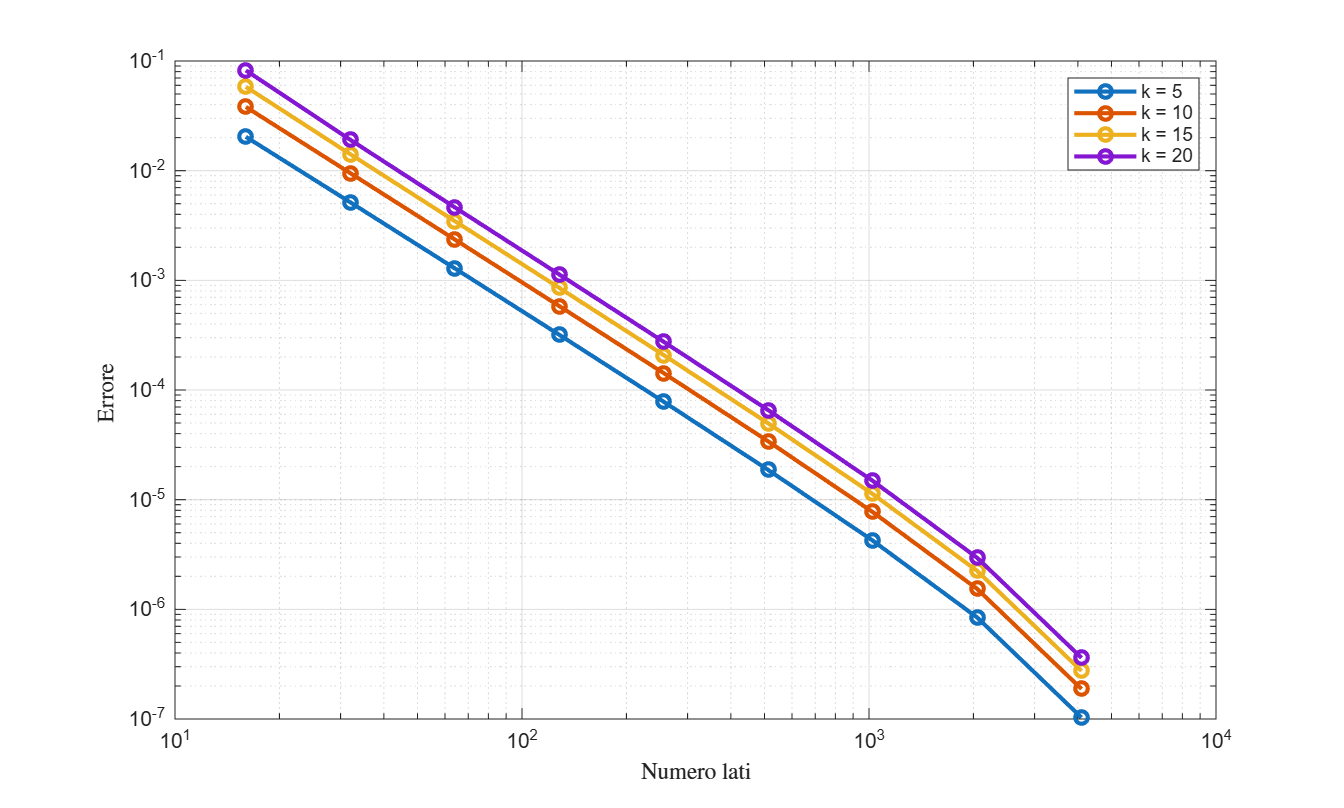
\includegraphics[width=\linewidth]{figures/ffp_approx_circ.png}
	\caption{Andamento dell'errore relativo tra il far field pattern analitico di una circonferenza di raggio $R=1$ e quello numerico. L'ostacolo è stato approssimato tramite poligoni regolari con numero di lati, coincidente con i gradi di libertà, pari a $16, 32, \dots, 4096$}
	\label{fig:ffp approx circonferenza}
\end{figure}


\subsection{Problemi inversi}
Nelle applicazioni fisiche reali (quali ad esempio sistemi radar, sonar), può capitare che l'obiettivo principale non sia calcolare il campo scatterato a partire da un ostacolo noto (chiamato \textit{problema diretto}), bensì l'opposto: si desidera ricostruire la forma, la posizione e in generale le caratteristiche di un ostacolo incognito misurando l'onda scatterata. Questo prende il nome di \textit{problema inverso di scattering}. Dal momento che solitamente i sensori di ricezione sono posti a grande distanza dall'ostacolo rispetto rispetto alle dimensioni dell'ostacolo stesso, la quantità fisica misurabile è proprio il far field pattern. Quest'ultimo costituisce dunque il dato di partenza per il problema di scattering inverso. \\
Prima di iniziare a ragionare su metodi numerici per affrontare un problema inverso di questo tipo è naturale chiedersi se la sola conoscenza del far field permetta di identificare in modo  unico ad esempio la forma dell'ostacolo. In altre parole, esiste il rischio che due ostacoli di forma diversa producano esattamente lo stesso far field? La risposta a questa domanda è fornita dal Teorema di Schiffer (si veda ad esempio \cite{CK19} Theorem 5.1). Nel caso di un ostacolo \textit{sound-soft}, il teorema stabilisce che l'ostacolo è determinato in modo univoco se si conosce il far field $u_\infty$ per tutte le direzioni di osservazione $\phi$ e per tutte le possibili direzioni dell'onda piana incidente $u^{inc}$ ad un fissato numero d'onda $k$. Determinare in modo univoco l'ostacolo conoscendo il far field generato solo da un numero finito di onde piane incidenti è un problema matematico più complesso e in generale non garantito, a meno di non imporre delle ipotesi sulla geometria e sulle dimensioni massime dell'ostacolo. Per maggiori dettagli si può guardare \cite{CK19}, Section 5.\\
Nel lavoro svolto in questa relazione ci poniamo in condizioni ancora più restrittive rispetto alle ipotesi generali di unicità globale: assumeremo nota a priori la forma geometrica dell'ostacolo poligonale (nello specifico, un quadrato) e cercheremo di ricostruire unicamente i parametri geometrici essenziali, ovvero la lunghezza del lato e l'angolo di rotazione. Questo riconduce il problema inverso ad uno spazio di ricerca bidimensionale. Il nostro obiettivo è minimizzare l'errore relativo commesso in norma $L^2$, ovvero:
\begin{equation}
	\label{eq:ffp funzione da minimizzare}
	E(l, \alpha) = \frac{\|u_\infty(l, \alpha) - u^{Ref}\|_{L^2}}{\|u^{Ref}\|_{L^2}},
\end{equation}
in cui $l$ indica la lunghezza del lato del quadrato e $\alpha$ è l'angolo di rotazione. \\
Per minimizzare tale funzione obiettivo abbiamo fissato il numero d'onda $k=20$ e l'angolo di incidenza $\theta = 0$, abbiamo calcolato il far field per ostacoli target di dimensioni e orientazioni diverse, scegliendo valori per il lato $l \in \{0.5, 0.7, 1.5, 3.0\}$ e per angolo $\alpha \in \{0, \pi/18, \pi/4, \pi/3\}$. Lo spazio di ricerca per gli algoritmi di minimizzazione è stato delimitato imponendo i bounds $l \in [0.1, \, 5]$ e $\alpha \in [0, \pi/2]$. Per ognuna delle 16 istanze sono stati utilizzati due approcci di minimizzazione differenti:
\begin{itemize}
	\item Approccio ibrido: \textit{Surrogate optimization} + Nelder-Mead. \\
	Inizialmente si sfrutta un algoritmo globale (implementato tramite la funzione \texttt{surrogateopt} di MATLAB) che esplora lo spazio dei parametri costruendo un modello matematico approssimativo della funzione obiettivo \ref{eq:ffp funzione da minimizzare} per individuare una stima iniziale della soluzione. Tale punto viene poi utilizzato come configurazione di partenza per la funzione \texttt{fminsearch} la quale applica il metodo di Nelder-Mead per calcolare un punto di minimo con maggiore precisione. Per maggiori dettagli si può fare riferimento ad esempio \cite{SurrOpt} per l'algoritmo di ricerca globale e la sezione 9.5 di \cite{NelderMead} per l'algoritmo di Nelder-Mead.
	\item \textit{Particle swarm optimization} (PSO).\\
	Un algoritmo di ottimizzazione globale (tramite la funzione \texttt{particleswarm}) che genera una popolazione di possibili soluzioni in grado di muoversi e condividere informazioni all'interno dello spazio di ricerca. Per i test effettuati è stata considerata una popolazione di 100 individui. Per una descrizione esaustiva del metodo si veda \cite{PSO}
\end{itemize}
I risultati ottenuti sono mostrati nella Tabella \ref{tab:confronto problema inverso}. Dall'analisi dei dati mostrati nella tabella possiamo effettuare una serie di considerazioni sulle strategie di ottimizzazione adottate. \\
Per ostacoli di piccole dimensioni rispetto alla lunghezza d'onda, nello specifico con lato $l= 0.5$ e $l=0.7$, la funzione obiettivo mostra un comportamento più regolare che consente ad entrambi gli approcci di convergere con successo verso i parametri geometrici corretti. In queste istanze abbiamo errori in norma $L^2$ (si veda l'equazione \ref{eq:ffp funzione da minimizzare}) dell'ordine di $10^{-10}$. In queste istanze tuttavia, l'approccio ibrido si rivela essere nettamente superiore sotto il profilo del tempo computazionale necessario, arrivando a convergenza in tempi ridotti, spesso inferiore a due minuti, a fronte dei 20-25 minuti richiesti dal PSO per gestire l'evoluzione dell'intera popolazione di particelle.\\
All'aumentare delle dimensioni del lato di $\Gamma$ la forte non-linearità del problema di scattering inverso si accentua notevolmente e la funzione di errore presenta numerosi minimi locali nei quali l'approccio ibrido rischia di rimanere intrappolato. Questo accade ad esempio nelle tre istanze evidenziate in rosso nella tabella. In questi casi specifici, le 200 valutazioni globali concesse alla funzione \texttt{surrogateopt} non si sono rivelate sufficienti per individuare la corretta regione di convergenza; di conseguenza l'algoritmo locale \texttt{fminsearch} ha raffinato la ricerca intorno ad un minimo locale errato, arrestandosi con un errore residuo dell'ordine di $10^{-1}$. Al contrario, l'algoritmo di PSO dimostra di essere più robusto sulle istanze considerate, risolvendole tutte correttamente. La comunicazione globale tra le particelle e l'ampia esplorazione stocastica dello spazio di ricerca permettono di non rimanere intrappolati in minimi locali ed arrivando sempre ad un errore finale dell'ordine di $10^{-11}$, pagando tuttavia a livello di tempo computazionale impiegato. 


\begin{table}[htbp]
	\centering
	\small 
	\begin{tabular}{cc | cccc | cccc}
		\toprule
		\multicolumn{2}{c}{\textbf{Target}} & \multicolumn{4}{c}{\textbf{fminsearch}} & \multicolumn{4}{c}{\textbf{Particle swarm}} \\
		\cmidrule(lr){1-2} \cmidrule(lr){3-6} \cmidrule(lr){7-10}
		$l$ & $\alpha$ & $l$ & $\alpha$ & Errore $L^2$ & Tempo (s) & $l$ & $\alpha$ & Errore $L^2$ & Tempo (s) \\
		\midrule
		0.5 & 0 & 0.5 & 0 & $1.92 \times 10^{-10}$ & 79.7  & 0.5 & 0 & $9.37 \times 10^{-12}$ & 580.5 \\
		0.5 & $\pi/18$ & 0.5 & $\pi/18$ & $1.56 \times 10^{-10}$ & 67.0  & 0.5 & $\pi/18$ & $2.96 \times 10^{-11}$ & 1207.4 \\
		0.5 & $\pi/4$ & 0.5 & $\pi/4$ & $2.00 \times 10^{-10}$ & 74.6  & 0.5 & $\pi/4$ & $2.18 \times 10^{-11}$ & 1248.2 \\
		0.5 & $\pi/3$ & 0.5 & $\pi/3$ & $1.19 \times 10^{-10}$ & 69.9  & 0.5 & $\pi/3$ & $3.48 \times 10^{-11}$ & 1484.7 \\
		\addlinespace
		0.7 & 0 & 0.7 & 0 & $1.97 \times 10^{-10}$ & 69.1  & 0.7 & 0 & $3.57 \times 10^{-11}$ & 1412.9 \\
		0.7 & $\pi/18$ & 0.7 & $\pi/18$ & $1.82 \times 10^{-10}$ & 175.7 & 0.7 & $\pi/18$ & $7.47 \times 10^{-11}$ & 1646.9 \\
		0.7 & $\pi/4$ & 0.7 & $\pi/4$ & $8.77 \times 10^{-11}$ & 109.0 & 0.7 & $\pi/4$ & $7.81 \times 10^{-11}$ & 1657.0 \\
		0.7 & $\pi/3$ & 0.7 & $\pi/3$ & $1.03 \times 10^{-10}$ & 95.5  & 0.7 & $\pi/3$ & $6.91 \times 10^{-11}$ & 1533.0 \\
		\addlinespace
		1.5 & 0 & 1.5 & 0 & $3.29 \times 10^{-10}$ & 75.2  & 1.5 & 0 & $7.85 \times 10^{-11}$ & 593.3 \\
		1.5 & $\pi/18$ & 1.5 & $\pi/18$ & $6.95 \times 10^{-11}$ & 63.2  & 1.5 & $\pi/18$ & $9.81 \times 10^{-11}$ & 719.6 \\
		1.5 & $\pi/4$ & 0.6 & $\pi/4$ & \textcolor{red}{$7.95 \times 10^{-1}$}  & 63.8  & 1.5 & $\pi/4$ & $2.57 \times 10^{-11}$ & 852.4 \\
		1.5 & $\pi/3$ & 1.5 & $\pi/3$ & $1.31 \times 10^{-10}$ & 64.4  & 1.5 & $\pi/3$ & $5.35 \times 10^{-11}$ & 1001.1 \\
		\addlinespace
		3.0 & 0 & 3.6 & 0 & \textcolor{red}{$5.06 \times 10^{-1}$}  & 51.9  & 3.0 & 0 & $2.48 \times 10^{-11}$ & 357.3 \\
		3.0 & $\pi/18$ & 3.0 & $\pi/18$ & $2.45 \times 10^{-10}$ & 59.1  & 3.0 & $\pi/18$ & $9.95 \times 10^{-11}$ & 1603.8 \\
		3.0 & $\pi/4$ & 2.6 & $\pi/4$ & \textcolor{red}{$3.81 \times 10^{-1}$}  & 64.4  & 3.0 & $\pi/4$ & $7.36 \times 10^{-11}$ & 1031.7 \\
		3.0 & $\pi/3$ & 3.0 & $\pi/3$ & $8.22 \times 10^{-11}$ & 81.1  & 3.0 & $\pi/3$ & $5.74 \times 10^{-11}$ & 1403.8 \\
		\bottomrule
	\end{tabular}
	\caption{Confronto tra le performance dell'algoritmo fminsearch e Particle Swarm.}
	\label{tab:confronto problema inverso}
\end{table}
\newpage
\printbibliography
\end{document}